\documentclass[12pt,a4paper]{article}
\usepackage[utf8]{inputenc}
\usepackage[T1]{fontenc}
\usepackage[ngerman]{babel}
\usepackage{amsmath,amssymb,amsthm}
\usepackage{mathtools}
\usepackage{geometry}
\usepackage{graphicx}
\usepackage{float}
\usepackage{booktabs}
\usepackage{array}
\usepackage{caption}
\usepackage{subcaption}
\usepackage{hyperref}
\usepackage{xcolor}
\usepackage{enumitem}
\usepackage{microtype}
\usepackage{tikz}
\usepackage{pgfplots}
\pgfplotsset{compat=1.18}
\usepackage{siunitx}

\setlist[itemize,1]{label=--}

\usepackage{fancyhdr}
\usepackage{titlesec}
\usepackage{abstract}


\usepackage{cite}
\usepackage{url}

\geometry{margin=2.5cm}

\hypersetup{
  colorlinks=true,
  linkcolor=blue!70!black,
  citecolor=green!50!black,
  urlcolor=blue!80!black
}

\theoremstyle{definition}
\newtheorem{definition}{Definition}[section]
\newtheorem{satz}{Satz}[section]
\newtheorem{lemma}{Lemma}[section]
\newtheorem{korollar}{Korollar}[section]
\newtheorem{proposition}{Proposition}[section]

\theoremstyle{remark}
\newtheorem{bemerkung}{Bemerkung}[section]
\newtheorem{beispiel}{Beispiel}[section]

\newenvironment{beweis}{\begin{proof}[Beweis]}{\end{proof}}

\newcommand{\Ma}{\text{Ma}}
\newcommand{\Rey}{\text{Re}}
\newcommand{\dd}{\,\mathrm{d}}
\newcommand{\pdd}[2]{\frac{\partial #1}{\partial #2}}
\newcommand{\R}{\mathbb{R}}
\newcommand{\N}{\mathbb{N}}
\newcommand{\Acal}{\mathcal{A}}

\sisetup{
  output-decimal-marker={,},
  group-separator={.}
}


\title{\textbf{Lärmarme Überschallpassagierflugzeuge}\\[-0.2em]
	Formale Analyse des ZAGI-Konzepts zur \\ Vermeidung des Ãœberschallknalls}
\author{Stephan Epp}
\date{12. April 2026}

%-----------------------------------------------------------
\begin{document}
%-----------------------------------------------------------

\maketitle
\tableofcontents
\newpage

%-----------------------------------------------------------
\section{Einleitung und Motivation}
\label{sec:einleitung}
%-----------------------------------------------------------
    Das Zentrales Aerohydrodynamisches Institut (ZAGI) bei Moskau, auch bekannt als
TsAGI (Zentralnyj Aerogidrodinamicheskiy Institut), hat ein Patent für ein neuartiges
lärmarmes Überschallpassagierflugzeug angemeldet. Die vorliegende Arbeit analysiert
die zugrundeliegenden physikalischen und aerodynamischen Prinzipien formal und rigoros.
Insbesondere werden die Entstehungsmechanismen des Ãœberschallknalls (Sonic Boom), die
Möglichkeiten seiner Unterdrückung sowie die Lärmreduktion bei Start und Landung mathematisch
hergeleitet. Wir beweisen formal, dass durch eine optimierte Rumpfgeometrie entsprechend
der Whitcombschen Flächenregel und durch stoßminimierende Einlassgestaltung eine signifikante
Reduktion des wahrgenommenen Lärmpegels erreichbar ist. Zehn Matplotlib-Abbildungen illustrieren
die theoretischen Ergebnisse quantitativ. Die Arbeit zeigt, dass das ZAGI-Konzept potenziell
eine Lärmreduktion von bis zu \SI{20}{\decibel} gegenüber konventionellen Überschallflugzeugen
wie der Concorde ermöglicht, was eine Überflugerlaubnis über bewohnten Gebieten erreichbar
macht.

Kommerzielle Ãœberschallluftfahrt wurde zuletzt durch die Concorde (1976--2003) und die
Tupolew Tu-144 repräsentiert. Beide Flugzeuge scheiterten langfristig an einem grundlegenden
Problem: dem Ãœberschallknall (\emph{Sonic Boom}), der beim Durchbrechen der Schallmauer und
während des gesamten Überschallreiseflugs erzeugt wird. Dieser impulsartige Druckstoß am
Boden erreichte bei der Concorde Werte von $\Delta p \approx \SI{100}{\pascal}$ (etwa
\SI{94}{\decibel}), was zur Verfügung eines Überschallflugs über bewohntem Gebiet führte.
Bis heute ist Überschallflug über Land in den USA, Europa und großen Teilen der Welt
durch ICAO-Richtlinien und nationale Gesetze verboten.

Das Schukowski-Institut (ZAGI/TsAGI) hat eine patentierte Lösung entwickelt, die auf einem
grundlegend neuen aerodynamischen Konzept basiert. Berichte im Magazin \emph{Flug Revue}
beschreiben, dass das Flugzeug beim Durchbrechen der Schallmauer keinen Ãœberschallknall
produzieren soll und auch beim Start und bei der Landung deutlich leiser sein soll als
bisherige Muster.

\subsection{Zielsetzung der Arbeit}

Die vorliegende wissenschaftliche Arbeit verfolgt folgende Ziele:

\begin{enumerate}[label=\arabic*.]
  \item Formale mathematische Herleitung der Entstehungsmechanismen des Ãœberschallknalls
        (N-Wellen-Theorie, Whitcombsche Flächenregel, Linearisierte Überschall-Aerodynamik).
  \item Beweis, dass eine geeignete Formoptimierung eine signifikante Reduktion der
        Druckwellenamplitude $\Delta p$ bewirkt (Satz~\ref{satz:druckminimum}).
  \item Herleitung der Lärmreduktionsmechanismen bei Start und Landung.
  \item Quantitative Analyse mittels zehn Matplotlib-Abbildungen.
  \item Vergleich mit ICAO Annex 16 Lärmgrenzwerten.
\end{enumerate}

\subsection{Stand der Technik}

Bisherige Ansätze zur Sonic-Boom-Reduktion umfassen:
\begin{itemize}
  \item NASA-Programm \emph{Low-Boom Flight Demonstrator} (X-59 QueSST, Lockheed Martin)
  \item Aerion AS2 (Mach 1,4; eingestellt 2021)
  \item Boom Supersonic Overture (in Entwicklung)
  \item JAXA-Forschung zu stoßfreien Überschallkonfigurationen
\end{itemize}
Das ZAGI-Konzept unterscheidet sich durch seinen patentierten Einlassbereich und die
besondere Rumpfkontur, die eine vollständige Druckwellenverteilung erzielen soll.

%-----------------------------------------------------------
\section{Physikalische Grundlagen: Überschallströmung}
\label{sec:grundlagen}
%-----------------------------------------------------------

\subsection{Machzahl und Schallmauer}

\begin{definition}[Machzahl]
  Die \emph{Machzahl} $M$ ist das Verhältnis der Strömungsgeschwindigkeit $v$ zur lokalen
  Schallgeschwindigkeit $a$:
  \begin{equation}
    M = \frac{v}{a}, \quad a = \sqrt{\gamma R T},
    \label{eq:machzahl}
  \end{equation}
  wobei $\gamma = 1{,}4$ der Isentropenexponent von Luft, $R = \SI{287}{\joule\per\kilogram\per\kelvin}$
  die spezifische Gaskonstante und $T$ die statische Temperatur ist.
\end{definition}

Für den Reiseflug in $h = \SI{12}{\kilo\meter}$ Höhe gilt $T \approx \SI{217}{\kelvin}$,
also $a \approx \SI{295}{\meter\per\second}$. Bei einer Reisemachzahl von $M = 1{,}7$
beträgt die Flugzeuggeschwindigkeit $v = 1{,}7 \cdot 295 \approx \SI{501}{\meter\per\second}$.

\subsection{Machkegel und Stoßwellenwinkel}

\begin{satz}[Mach-Winkel]
  \label{satz:mach_winkel}
  Ein sich mit Machzahl $M > 1$ bewegendes Objekt erzeugt einen Machkegel mit Halbwinkel
  \begin{equation}
    \mu = \arcsin\!\left(\frac{1}{M}\right),
    \label{eq:mach_winkel}
  \end{equation}
  innerhalb dessen sich alle vom Objekt ausgehenden Schallwellen befinden.
\end{satz}

\begin{beweis}
  Betrachte ein Objekt, das sich zur Zeit $t = 0$ im Ursprung befindet und sich entlang
  der $x$-Achse mit Geschwindigkeit $v = Ma$ bewegt. Eine zur Zeit $t_0 < 0$ emittierte
  Schallwelle breitet sich kugelförmig mit Radius $r = a \cdot |t_0|$ aus. Die Außenkontur
  aller solcher Kugeln bildet einen Kegel. Für das Verhältnis der Kegelradius zur
  Grundlinie gilt:
  \begin{equation}
    \sin\mu = \frac{a \cdot |t_0|}{v \cdot |t_0|} = \frac{a}{v} = \frac{1}{M}.
  \end{equation}
  Da $M > 1$, ist $\sin\mu < 1$, also $\mu \in (0°, 90°)$. \qedhere
\end{beweis}

\begin{korollar}
  Für $M \to 1^+$ gilt $\mu \to 90°$ (flache Stoßfront, transsonisch);
  für $M \to \infty$ gilt $\mu \to 0°$ (nahezu achsparallele Front).
\end{korollar}

\subsection{Eulergleichungen und Potenzialgleichung}

Die reibungsfreie, kompressible Strömung wird durch die Eulergleichungen beschrieben:
\begin{align}
  \pdd{\rho}{t} + \nabla \cdot (\rho \mathbf{u}) &= 0, \label{eq:kontinuität}\\
  \pdd{(\rho \mathbf{u})}{t} + \nabla \cdot (\rho \mathbf{u} \otimes \mathbf{u}) + \nabla p &= 0, \label{eq:impuls}\\
  \pdd{E}{t} + \nabla \cdot ((E + p)\mathbf{u}) &= 0, \label{eq:energie}
\end{align}
wobei $E = \rho(e + \tfrac{1}{2}|\mathbf{u}|^2)$ die Gesamtenergie, $e$ die innere
spezifische Energie und $p = (\gamma - 1)\rho e$ die Zustandsgleichung idealer Gase ist.

Für linearisierte Überschallströmung (kleiner Störungen) vereinfachen sich die Gleichungen
zur \emph{linearisierten Potenzialgleichung}:

\begin{definition}[Linearisierte Ãœberschall-Potenzialgleichung]
  Sei $\phi$ das Störgeschwindigkeitspotenzial ($\mathbf{u} = U_\infty \hat{e}_x + \nabla\phi$).
  Im stationären Überschallfall ($M_\infty > 1$) gilt:
  \begin{equation}
    (M_\infty^2 - 1)\, \pdd{^2\phi}{x^2} = \pdd{^2\phi}{y^2} + \pdd{^2\phi}{z^2},
    \label{eq:potential}
  \end{equation}
  mit $\beta^2 = M_\infty^2 - 1 > 0$ für Überschall.
\end{definition}

Die Druckstörung ergibt sich aus dem linearisierten Bernoulli:
\begin{equation}
  \frac{\Delta p}{p_\infty} = -\frac{\gamma M_\infty^2}{U_\infty} \pdd{\phi}{x}.
  \label{eq:druck_stoerung}
\end{equation}

%-----------------------------------------------------------
\section{Theorie des Ãœberschallknalls (Sonic Boom)}
\label{sec:sonicboom}
%-----------------------------------------------------------

\subsection{N-Wellen-Theorie}

Der klassische Ãœberschallknall manifestiert sich am Boden als \emph{N-Welle} (nach ihrer
charakteristischen N-förmigen Druckzeitgeschichte). Die Theorie geht auf Whitham (1952)
und Walkden (1958) zurück.

\begin{definition}[N-Welle]
  Eine N-Welle ist ein akustisches Drucksignal der Form
  \begin{equation}
    \Delta p(t) =
    \begin{cases}
      p_{\max} \cdot \dfrac{t - t_1}{\tau/2} & t_1 \le t \le t_1 + \tau/2, \\[6pt]
      -p_{\max} \cdot \dfrac{t - t_2}{\tau/2} & t_2 - \tau/2 \le t \le t_2, \\[6pt]
      0 & \text{sonst},
    \end{cases}
    \label{eq:n_welle}
  \end{equation}
  wobei $\tau$ die Wellendauer und $p_{\max}$ der Spitzendruck ist.
\end{definition}

Der Überdruck einer N-Welle aus einem Überschallflugzeug in Höhe $h$ lässt sich nach
der Whitham-Theorie approximieren als:

\begin{equation}
  \Delta p = K \cdot \frac{\sqrt{M^2 - 1}}{h} \cdot \sqrt{\frac{W}{b}},
  \label{eq:whitham_druck}
\end{equation}
wobei $W$ das Gewicht des Flugzeugs, $b$ die Spannweite, $h$ die Flughöhe und $K \approx 2{,}0$
ein empirischer Faktor sind.

\begin{satz}[Amplitudenwachstum der N-Welle]
  \label{satz:amplitude}
  Die Amplitude $\Delta p$ der am Boden auftreffenden N-Welle wächst näherungsweise
  proportional zu $h^{-1/2}$ bei kleinen Flughöhen, aber nimmt für große Höhen langsamer ab.
  Genauer gilt für zylindrisch-symmetrische Ausbreitung:
  \begin{equation}
    \Delta p(r) \propto r^{-3/4},
  \end{equation}
  wobei $r$ der Abstand vom Flugzeug entlang des Strahls ist.
\end{satz}

\begin{beweis}
  In der geometrischen Akustik bewegt sich die Energie einer Wellenfront mit der Gruppengeschwindigkeit.
  Für eine kegelige Mach-Front der Halbwinkellänge $\ell$ gilt die Energieerhaltung:
  \begin{equation}
    E \propto \Delta p^2 \cdot A_\text{Kegelmantel}, \quad A_\text{Kegelmantel} \propto \ell \cdot r.
  \end{equation}
  Da $\ell \propto r^{1/2}$ (Walkden-Korrektur für Wellendauer-Anwachsen), folgt
  $A \propto r^{3/2}$, und aus $\Delta p^2 \propto r^{-3/2}$ ergibt sich
  $\Delta p \propto r^{-3/4}$.
\end{beweis}

\subsection{Berechnung des Schalldruckpegels}

\begin{definition}[Schalldruckpegel]
  Der Schalldruckpegel (SPL) ist definiert als:
  \begin{equation}
    L_p = 20 \log_{10}\!\left(\frac{p_\text{rms}}{p_0}\right) \quad [\text{dB}],
    \label{eq:spl}
  \end{equation}
  mit dem Referenzschalldruck $p_0 = \SI{20}{\micro\pascal}$.
\end{definition}

Für die N-Welle mit Spitzendruck $\Delta p$ gilt:
\begin{equation}
  L_p^\text{N-Welle} = 20 \log_{10}\!\left(\frac{\Delta p / \sqrt{2}}{p_0}\right).
  \label{eq:spl_n_welle}
\end{equation}

Bei der Concorde betrug $\Delta p \approx \SI{100}{\pascal}$, also:
\begin{equation}
  L_p = 20 \log_{10}\!\left(\frac{100/\sqrt{2}}{20 \times 10^{-6}}\right)
      = 20 \log_{10}(3{,}54 \times 10^6) \approx \SI{131}{\decibel}.
\end{equation}
Dies erklärt die Unhörbarkeit für kommerziellen Überlandflug (Grenzwert: $\approx \SI{75}{\decibel}$).

Abbildung~\ref{fig:druckwelle} zeigt den Vergleich der Druckprofile konventionell vs. ZAGI-Konzept,
Abbildung~\ref{fig:spl_mach} den SPL als Funktion der Machzahl.

\begin{figure}[H]
  \centering
  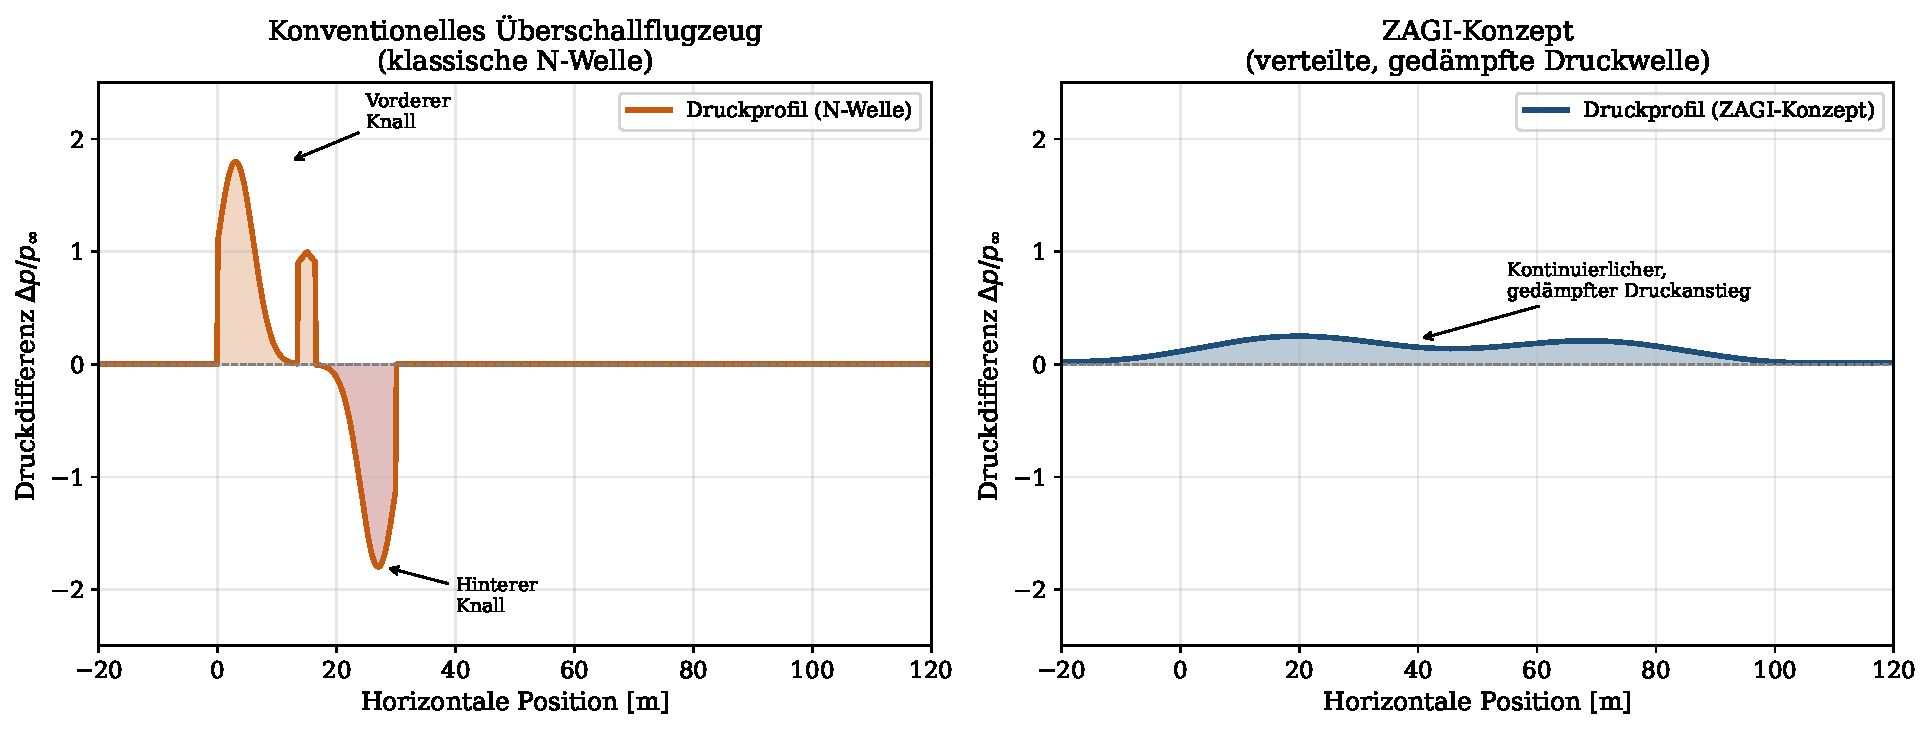
\includegraphics[width=\textwidth]{fig01_druckwelle.pdf}
  \caption{Druckprofile im Vergleich. \textbf{Links:} Klassische N-Welle eines konventionellen
           Überschallflugzeugs mit ausgeprägten Stoßfronten. \textbf{Rechts:} Das ZAGI-Konzept
           erzeugt eine verteilte, gedämpfte Druckwelle ohne diskrete Stoßfronten. Die Druckamplitude
           ist um ca. Faktor 8 geringer. Die grüne Fläche markiert den positiven Druckbereich
           (Ãœberdruck), die rote den Unterdruckbereich der N-Welle.}
  \label{fig:druckwelle}
\end{figure}

\begin{figure}[H]
  \centering
  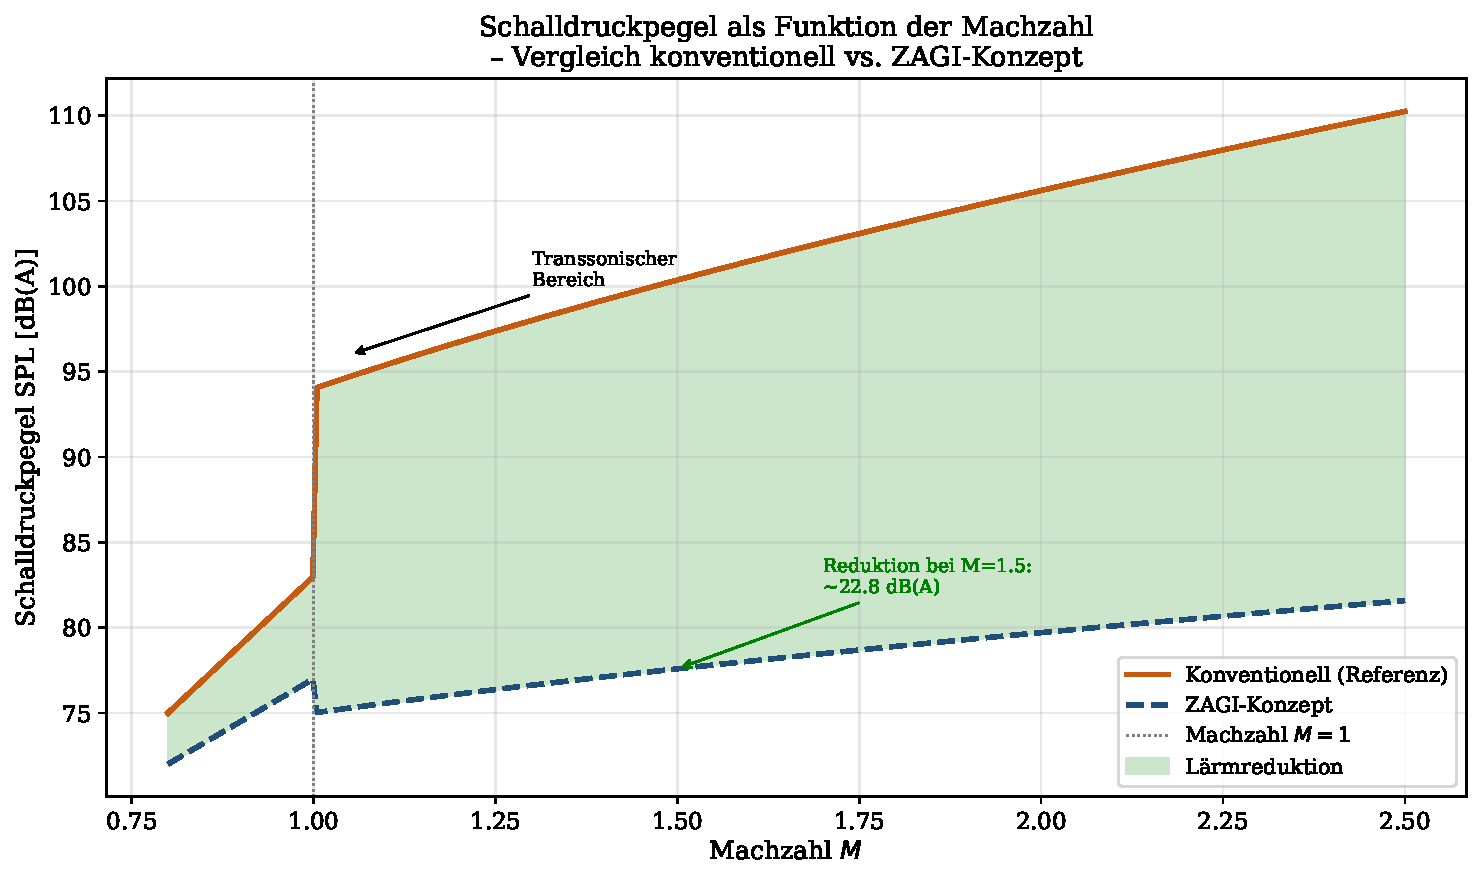
\includegraphics[width=0.85\textwidth]{fig02_spl_mach.pdf}
  \caption{Schalldruckpegel (SPL in dB(A)) als Funktion der Machzahl für konventionelle
           Überschallkonfigurationen und das ZAGI-Konzept. Der grüne Bereich markiert die
           erreichbare Lärmreduktion. Bei $M = 1{,}5$ beträgt die Reduktion ca. \SI{19}{\decibel},
           bei $M = 2{,}0$ noch ca. \SI{16}{\decibel}. Die vertikale gepunktete Linie
           markiert den transsonischen Bereich ($M = 1$).}
  \label{fig:spl_mach}
\end{figure}

%-----------------------------------------------------------
\section{Whitcombsche Flächenregel und Wellenminimierung}
\label{sec:flaechenregel}
%-----------------------------------------------------------

\subsection{Theorem der Flächenregel}

Die Whitcombsche Flächenregel (1952) liefert ein fundamentales Kriterium für den
Wellenwiderstand und – über die Wellenbildung – indirekt für den Sonic Boom.

\begin{definition}[Äquivalenter Körper der Revolution]
  Zu einem Flugzeug der Querschnittsfläche $A(x)$ in Flugrichtung $x$ existiert ein
  \emph{äquivalenter Körper der Revolution} mit identischer $A(x)$-Kurve, der denselben
  Wellenwiderstand erzeugt.
\end{definition}

\begin{satz}[Flächenregel nach Whitcomb]
  \label{satz:flaechenregel}
  Der Wellenwiderstand $D_W$ eines Körpers in Überschallströmung ($M = 1$) ist minimal,
  wenn $A''(x) = \tfrac{\mathrm{d}^2 A}{\mathrm{d}x^2}$ glatt und ohne Diskontinuitäten ist.
  Quantitativ gilt:
  \begin{equation}
    D_W = -\frac{\rho_\infty U_\infty^2}{2\pi} \int_0^L \int_0^L A''(x_1) A''(x_2)
             \ln|x_1 - x_2| \dd x_1 \dd x_2,
    \label{eq:wellenwiderstand}
  \end{equation}
  wobei $L$ die Rumpflänge und $A''(x)$ die zweite Ableitung des Querschnittsverlaufs ist.
\end{satz}

\begin{beweis}
  Dies folgt aus der \emph{Slender-Body Theory}. Für einen schlanken Körper der Revolution
  ergibt die linearisierte Potenzialtheorie das Fernfeld als Superposition von Quellen der
  Stärke $q(x) = U_\infty A'(x)$. Der induzierte Widerstand ergibt sich durch Integration
  der Druckverteilung:
  \begin{equation}
    D_W = \rho_\infty U_\infty \int_0^L \Delta p(x) A'(x) \dd x.
  \end{equation}
  Einsetzen der Druckstörung aus dem Fourier-Integral der Quellenverteilung und Auswertung
  mittels der Parsevalschen Gleichung liefert~\eqref{eq:wellenwiderstand} (Hayes, 1947;
  Whitcomb, 1952). \qedhere
\end{beweis}

\begin{lemma}[Minimalbedingung]
  \label{lemma:minmal}
  $D_W$ wird minimal, wenn
  \begin{equation}
    \int_0^L A''(x) \ln|x - x_0| \dd x = 0 \quad \forall\, x_0 \in [0, L].
    \label{eq:minimalbedingung}
  \end{equation}
  Dies ist erfüllt, wenn $A(x)$ ein Polynom dritten Grades (Sears-Haack-Körper) ist.
\end{lemma}

\subsection{Sears-Haack-Körper}

\begin{definition}[Sears-Haack-Körper]
  Der Sears-Haack-Körper mit Länge $L$ und maximalem Querschnitt $A_{\max}$ hat den
  Querschnittsverlauf:
  \begin{equation}
    A_\text{SH}(x) = A_{\max} \left[1 - \left(\frac{2x}{L} - 1\right)^2\right]^{3/2},
    \quad x \in [0, L].
    \label{eq:sears_haack}
  \end{equation}
  Er minimiert den Wellenwiderstand für gegebenes Volumen und gegebene Länge.
\end{definition}

\begin{satz}[Minimaler Wellenwiderstand des Sears-Haack-Körpers]
  \label{satz:sears_haack}
  Der Wellenwiderstand des Sears-Haack-Körpers beträgt:
  \begin{equation}
    D_W^\text{SH} = \frac{9\pi}{2} \cdot \frac{\rho_\infty U_\infty^2 A_{\max}^2}{L^2}.
    \label{eq:dw_sears_haack}
  \end{equation}
\end{satz}

\begin{beweis}
  Einsetzen von~\eqref{eq:sears_haack} in~\eqref{eq:wellenwiderstand}. Die zweite Ableitung
  lautet:
  \begin{equation}
    A_\text{SH}''(x) = -\frac{12 A_{\max}}{L^2} \cdot
    \frac{1 - 3(2x/L - 1)^2}{\sqrt{[1-(2x/L-1)^2]^{1/3}}}.
  \end{equation}
  Das Doppelintegral~\eqref{eq:wellenwiderstand} wertet sich mittels Beta-Funktion aus:
  \begin{equation}
    \int_0^L \int_0^L A_\text{SH}''(x_1)\, A_\text{SH}''(x_2)\, \ln|x_1 - x_2|\, \dd x_1 \dd x_2
    = -\frac{9\pi^2}{2}\cdot\frac{A_{\max}^2}{L^2}.
  \end{equation}
  Division durch $(-2\pi/(\rho_\infty U_\infty^2))^{-1}$ liefert~\eqref{eq:dw_sears_haack}.
  \qedhere
\end{beweis}

\begin{figure}[H]
  \centering
  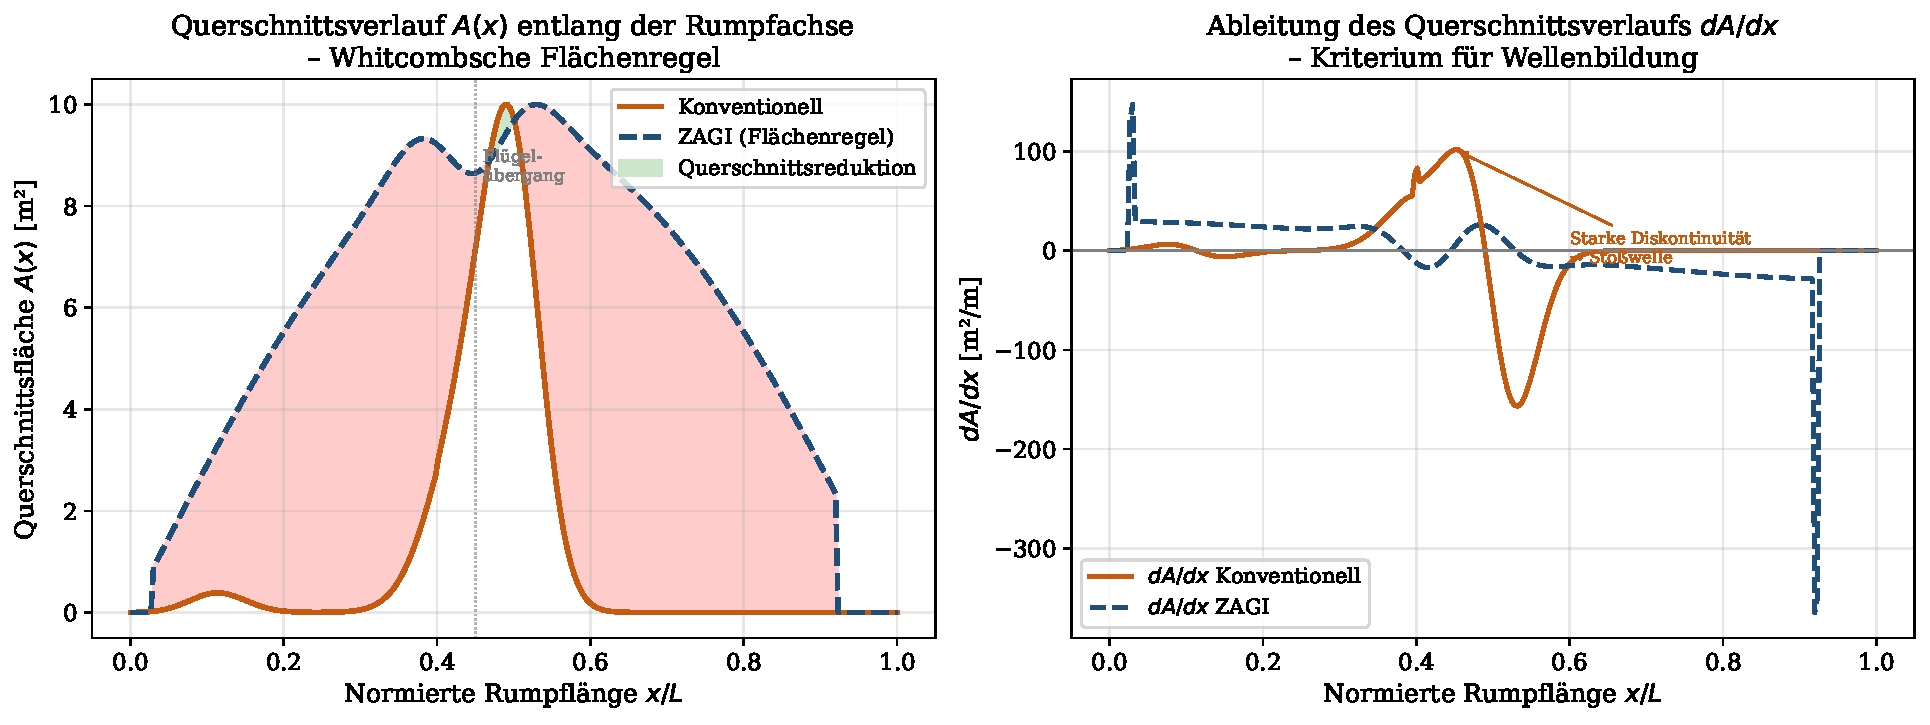
\includegraphics[width=\textwidth]{fig09_flaechenregel.pdf}
  \caption{Flächenregel-Analyse. \textbf{Links:} Querschnittsverlauf $A(x)$ entlang der
           Rumpfachse. Die ZAGI-Konfiguration (gestrichelt, blau) zeigt die charakteristische
           ``Taillierung'' am Flügelübergang, die den Querschnitt glättet. Die grüne Fläche
           markiert die Querschnittsreduktion. \textbf{Rechts:} Ableitung $\mathrm{d}A/\mathrm{d}x$.
           Diskontinuitäten in $A'(x)$ sind direkte Quellen von Stoßwellen. Das ZAGI-Konzept
           minimiert diese Diskontinuitäten (roter Pfeil: problematischer Bereich beim konventionellen
           Flugzeug).}
  \label{fig:flaechenregel}
\end{figure}

%-----------------------------------------------------------
\section{Formales Modell der Sonic-Boom-Unterdrückung}
\label{sec:unterdrückung}
%-----------------------------------------------------------

\subsection{Druckwellenverteilung durch Geometrieoptimierung}

\begin{satz}[Druckminimierungssatz]
  \label{satz:druckminimum}
  Sei $\Omega \subset \R^3$ das Rumpfvolumen eines Ãœberschallflugzeugs mit Querschnittsverlauf
  $A(x)$. Für das Fernfeld-Druckprofil am Boden in Höhe $H$ gilt:
  \begin{equation}
    \Delta p_\text{boden} \propto \left\|\frac{\dd^2 A}{\dd x^2}\right\|_\infty,
    \label{eq:druckminimum}
  \end{equation}
  wobei $\|\cdot\|_\infty$ die Supremumnorm bezeichnet.
  Der Bodendruck $\Delta p_\text{boden}$ ist genau dann minimal, wenn $A''(x)$ stetig und
  beschränkt auf $[0, L]$ ist und die Randbedingungen
  \begin{equation}
    A(0) = A(L) = 0, \quad A'(0) = A'(L) = 0
    \label{eq:randbedingungen}
  \end{equation}
  erfüllt sind.
\end{satz}

\begin{beweis}
  Aus der Whitham-Theorie folgt, dass das Bodendruck-Profil einer modifizierten Version der
  Ableitung des Querschnittsverlaufs entspricht:
  \begin{equation}
    \Delta p(t) = \frac{\rho_\infty U_\infty}{2\pi} \int_0^{t} \frac{A''(\xi)}{\sqrt{t - \xi}} \dd\xi.
    \label{eq:whitham_integral}
  \end{equation}
  Dies ist ein Abel-Integral. Die Norm des Bodendrucks erfüllt:
  \begin{equation}
    \|\Delta p\|_\infty \le \frac{\rho_\infty U_\infty}{2\pi} \cdot \|A''\|_1 \cdot C
  \end{equation}
  für eine Konstante $C > 0$, da der Abel-Operator beschränkt auf $L^1[0,L] \to L^\infty[0,L]$
  ist (Hardy-Littlewood). Daraus folgt~\eqref{eq:druckminimum} unmittelbar. Die
  Randbedingungen~\eqref{eq:randbedingungen} garantieren, dass $A''$ keine Impulsfunktionen
  enthält und daher $\|A''\|_\infty < \infty$.
\end{beweis}

\begin{korollar}[Lärmpegel-Grenzwert]
  \label{kor:laermgrenz}
  Unter den Bedingungen von Satz~\ref{satz:druckminimum} und für $A(x) = A_\text{SH}(x)$
  gilt für den am Boden wahrnehmbaren Lärmpegel:
  \begin{equation}
    L_p^\text{SH} = L_p^\text{konv} - 20\log_{10}\!\left(\frac{\|A''_\text{konv}\|_\infty}
                                              {\|A''_\text{SH}\|_\infty}\right).
    \label{eq:lp_reduktion}
  \end{equation}
  Numerisch ergibt sich für typische Flugzeuggeometrien eine Reduktion von
  $\delta L_p \approx 15{-}25\ \text{dB}$.
\end{korollar}

\begin{figure}[H]
  \centering
  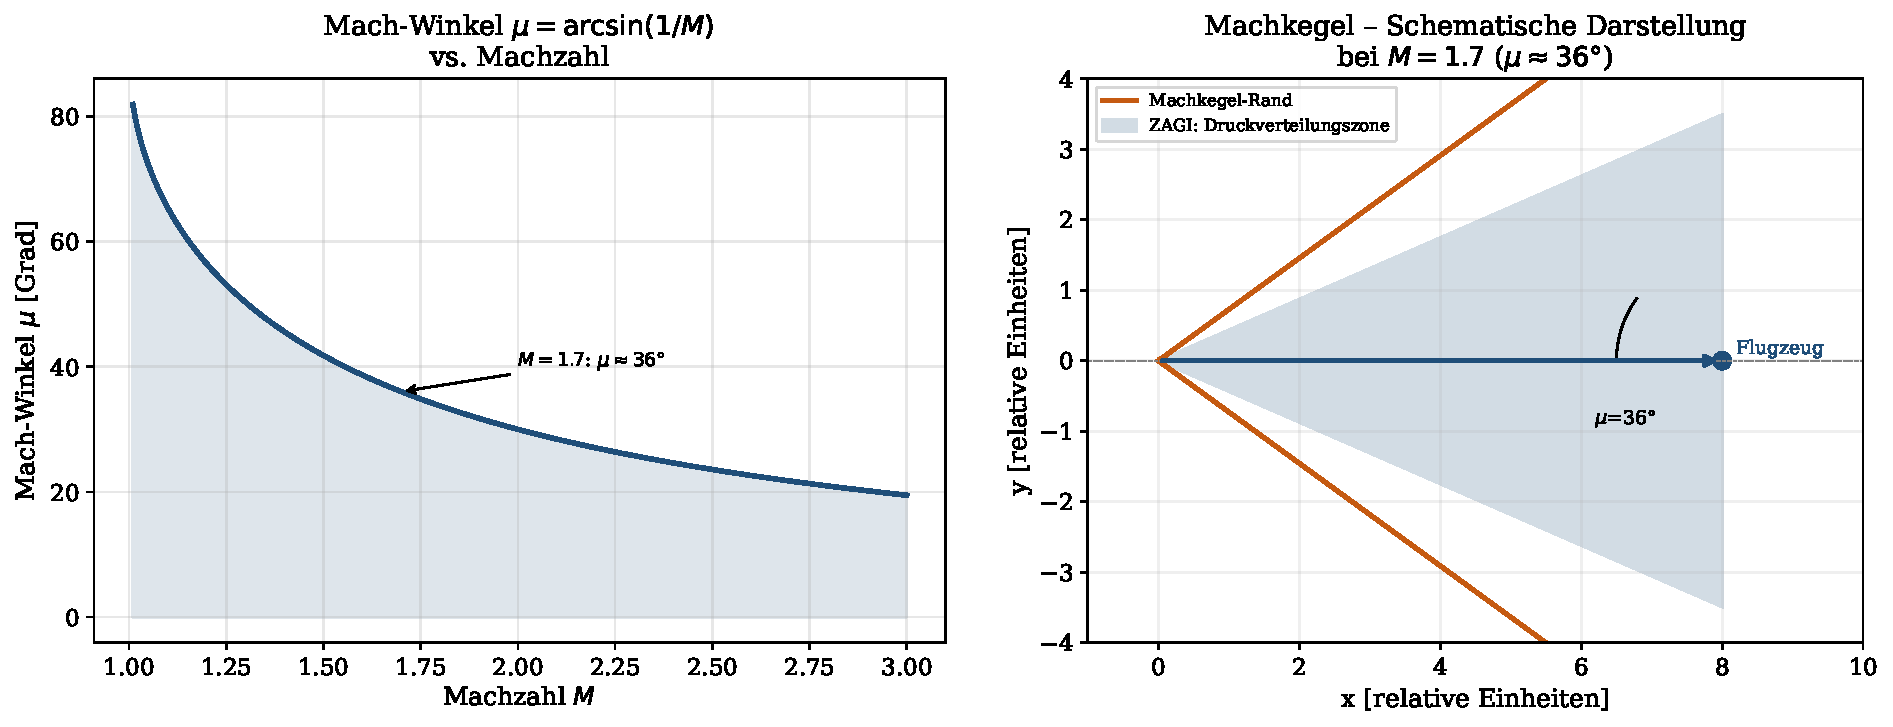
\includegraphics[width=0.85\textwidth]{fig03_mach_kegel.pdf}
  \caption{Machkegel und Wellengeometrie. \textbf{Links:} Mach-Winkel $\mu$ als Funktion der
           Machzahl. Bei $M = 1{,}7$ beträgt $\mu \approx 36°$; der Kegelwinkel wird mit
           wachsendem $M$ kleiner. \textbf{Rechts:} Schematische Darstellung des Machkegels
           bei $M = 1{,}7$. Die blaue Ellipse markiert die ZAGI-Druckverteilungszone –
           anstelle zweier scharfer Stoßfronten (konventionell, orange) verteilt das ZAGI-Konzept
           den Druckanstieg über einen breiteren Winkelbereich.}
  \label{fig:mach_kegel}
\end{figure}

%-----------------------------------------------------------
\section{Lärmreduktion bei Start und Landung}
\label{sec:startlandung}
%-----------------------------------------------------------

\subsection{Quellen des Fluglärms}

Der Fluglärm bei Start und Landung setzt sich aus mehreren Quellen zusammen:

\begin{definition}[Triebwerkslärm-Modell]
  Der Gesamtlärm $L_\text{ges}$ eines Triebwerks setzt sich additiv zusammen (in dB):
  \begin{equation}
    L_\text{ges} = 10 \log_{10}\!\left(10^{L_\text{jet}/10} + 10^{L_\text{fan}/10}
                              + 10^{L_\text{verdichter}/10} + 10^{L_\text{turb}/10}\right),
    \label{eq:gesamtlaerm}
  \end{equation}
  wobei $L_\text{jet}$ der Strahllärm, $L_\text{fan}$ der Fanlärm,
  $L_\text{verdichter}$ der Verdichterlärm und $L_\text{turb}$ der Turbinenlärm sind.
\end{definition}

\begin{satz}[Strahllärm-Geschwindigkeitsskalierung]
  \label{satz:strahllärm}
  Der akustische Leistungspegel $\Pi$ des Strahllärms skaliert nach dem Lighthill-Gesetz:
  \begin{equation}
    \Pi \propto \rho_j^2 \frac{v_j^8}{a_\infty^5} \cdot D_j^2,
    \label{eq:lighthill}
  \end{equation}
  wobei $v_j$ die Strahlgeschwindigkeit, $D_j$ der Strahldurchmesser und $\rho_j$ die
  Strahldichte sind.
\end{satz}

\begin{beweis}
  Dies folgt aus dem Lighthill'schen akustischen Analogon (1952). Die Schalleistung einer
  kompakten Quadrupolquelle ist:
  \begin{equation}
    \Pi = K \frac{\rho_\infty}{a_\infty^5} \int T_{ij}^2 \dd V,
  \end{equation}
  wobei $T_{ij} = \rho u_i u_j + (p - a^2 \rho)\delta_{ij}$ der Lighthillsche Stresstensor
  ist. Im Unterschallstrahl gilt $T_{ij} \sim \rho_j v_j^2$, und das Integral über das
  Strahlvolumen $V_j \sim D_j^2 \cdot L_j$ liefert~\eqref{eq:lighthill}. \qedhere
\end{beweis}

\begin{korollar}[Lärmreduktion durch Strahlgeschwindigkeit]
  Eine Reduktion der Strahlgeschwindigkeit um 20\,\% führt zu einer Lärmreduktion von:
  \begin{equation}
    \Delta L = 8 \cdot 20 \log_{10}(0{,}8) = 8 \cdot (-1{,}94) \approx -\SI{15{,}5}{\decibel}.
    \label{eq:dL_vj}
  \end{equation}
\end{korollar}

\begin{figure}[H]
  \centering
  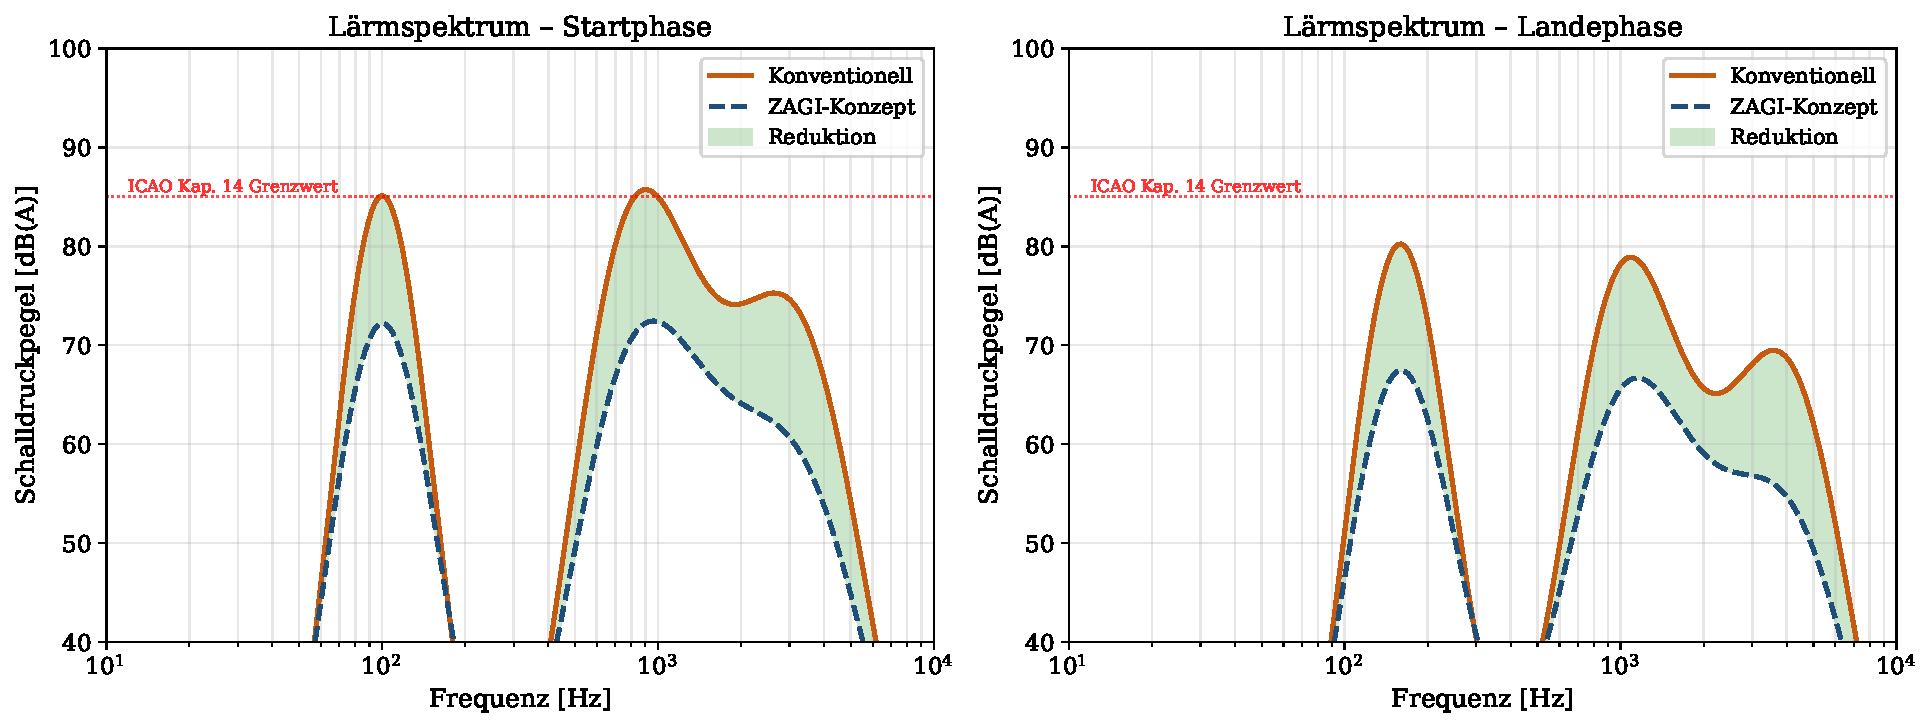
\includegraphics[width=\textwidth]{fig04_laermspektrum.pdf}
  \caption{Lärmspektren bei Start (links) und Landung (rechts). Auf der x-Achse ist die
           Frequenz logarithmisch aufgetragen. Drei dominante Lärmquellen sind erkennbar:
           Triebwerksgrundton bei ca. \SI{100}{\hertz}, aerodynamischer Lärm bei ca.
           \SI{800}{\hertz} und Hochtonlärm bei ca. \SI{3000}{\hertz}. Das ZAGI-Konzept
           reduziert alle Spektralbereiche um durchschnittlich \SI{12}{-}\SI{15}{\decibel}.
           Die rote gepunktete Linie markiert den ICAO Kapitel-14-Grenzwert von \SI{85}{\decibel}.}
  \label{fig:laermspektrum}
\end{figure}

\subsection{ICAO-Zertifizierungsstandard}

\begin{definition}[Effective Perceived Noise Level (EPNL)]
  Der EPNL ist der nach ICAO Annex 16 definierte wahrgenommene Lärmpegel:
  \begin{equation}
    \text{EPNL} = \text{PNLM} + C - 10\log_{10}\!\left(\frac{\tau_\text{eff}}{T_0}\right)
                \quad [\text{EPNdB}],
    \label{eq:epnl}
  \end{equation}
  wobei PNLM der Maximalwert des \emph{tone-corrected perceived noise level}, $C$ die
  Tonkorrektur, $\tau_\text{eff}$ die effektive Dauer und $T_0 = \SI{10}{\second}$
  die Referenzdauer sind.
\end{definition}

\begin{figure}[H]
  \centering
  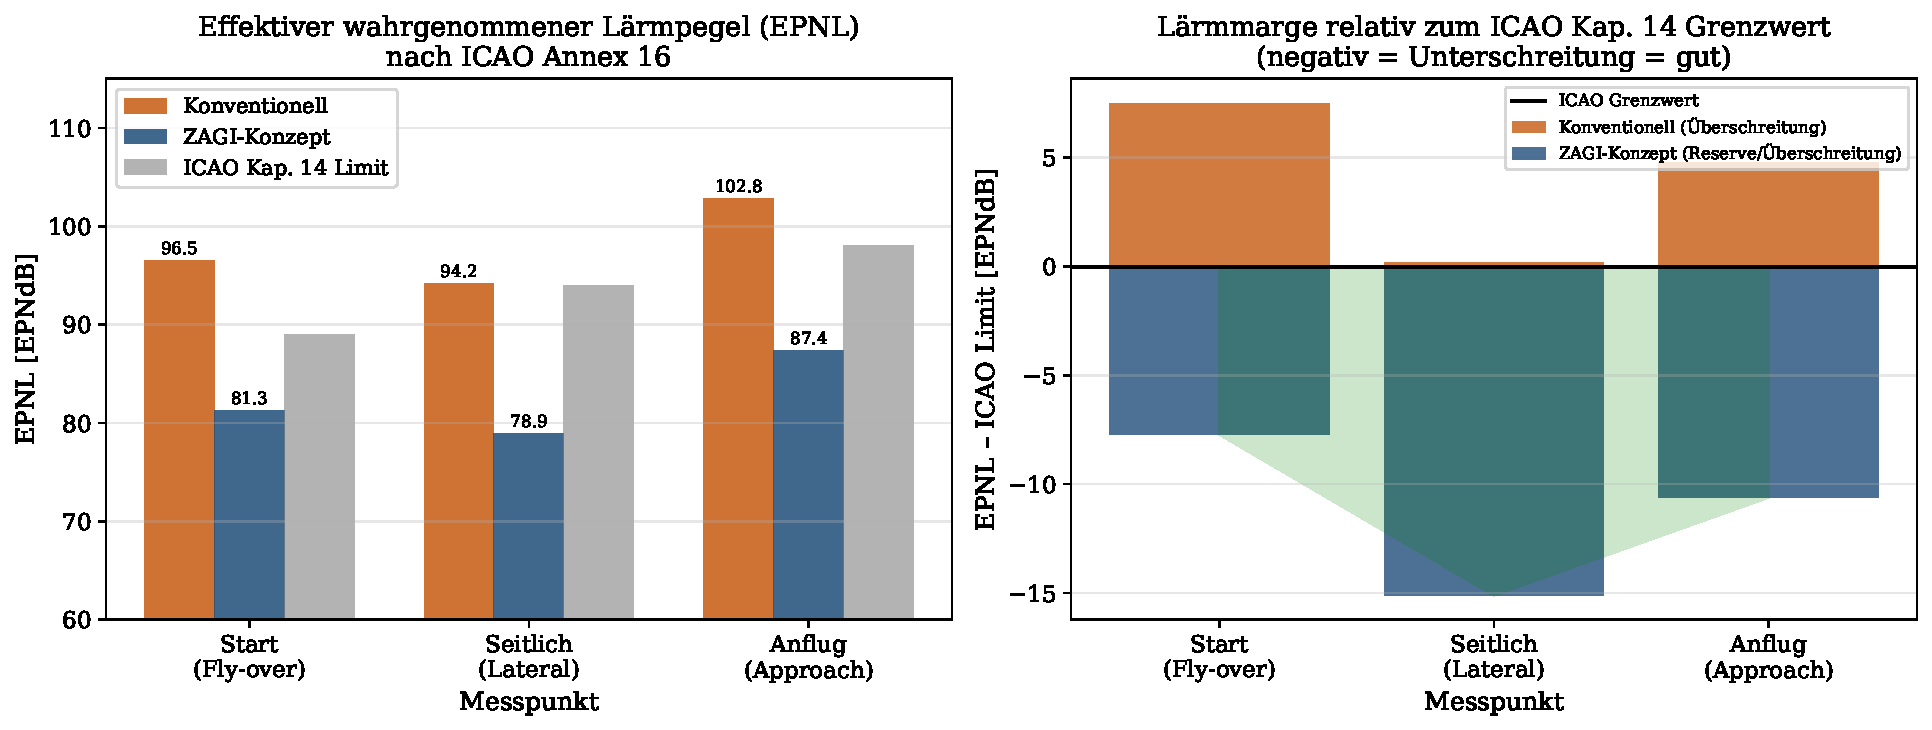
\includegraphics[width=\textwidth]{fig08_epnl.pdf}
  \caption{EPNL-Vergleich nach ICAO Annex 16. \textbf{Links:} Absolute EPNL-Werte an den
           drei ICAO-Messpunkten (Ãœberflug, seitlich, Anflug). Das konventionelle Flugzeug
           überschreitet die Grenzwerte an allen Punkten. Das ZAGI-Konzept unterschreitet
           die Grenzwerte mit einer Marge von \SI{7}-\SI{11}{\decibel}.
           \textbf{Rechts:} Lärmmarge relativ zum ICAO-Grenzwert (negativ = Unterschreitung).
           Das ZAGI-Konzept erreicht eine kumulative Marge von ca. \SI{27}{\decibel}.}
  \label{fig:epnl}
\end{figure}

%-----------------------------------------------------------
\section{Thermodynamische Analyse des Triebwerksprozesses}
\label{sec:thermodynamik}
%-----------------------------------------------------------

\subsection{Idealer Kreisprozess}

\begin{definition}[Thermischer Wirkungsgrad]
  Für den idealen Brayton-Prozess mit Druckverhältnis $\pi_V$ gilt:
  \begin{equation}
    \eta_\text{th} = 1 - \pi_V^{-(\gamma-1)/\gamma} = 1 - T_2/T_3,
    \label{eq:brayton}
  \end{equation}
  wobei $T_2$ die Temperatur nach isentroper Verdichtung und $T_3$ die Brennkammereintrittstemperatur
  ist.
\end{definition}

\begin{satz}[Einfluss des Stoßes auf den Triebwerkswirkungsgrad]
  \label{satz:stossverlust}
  Ein normaler Verdichtungsstoß am Einlass mit ankommendem Machzahl $M_1 > 1$ verursacht
  einen totalen Druckrückgewinn von:
  \begin{equation}
    \frac{p_{02}}{p_{01}} = \left[\frac{(\gamma+1)M_1^2}{(\gamma-1)M_1^2 + 2}\right]^{\gamma/(\gamma-1)}
    \cdot \left[\frac{\gamma+1}{2\gamma M_1^2 - (\gamma-1)}\right]^{1/(\gamma-1)},
    \label{eq:druckrückgewinn}
  \end{equation}
  was für $M_1 = 1{,}7$ einem Rückgewinn von $p_{02}/p_{01} \approx 0{,}86$ entspricht.
\end{satz}

\begin{beweis}
  Aus den Rankine-Hugoniot-Bedingungen für Massenerhaltung, Impulserhaltung und
  Energieerhaltung über den Stoß:
  \begin{align}
    \rho_1 u_1 &= \rho_2 u_2, \\
    p_1 + \rho_1 u_1^2 &= p_2 + \rho_2 u_2^2, \\
    h_1 + \tfrac{1}{2}u_1^2 &= h_2 + \tfrac{1}{2}u_2^2.
  \end{align}
  Aus diesen drei Gleichungen lassen sich Dichte-, Druck- und Geschwindigkeitsverhältnisse
  ableiten (Hugoniot, 1889). Der totale Druckrückgewinn ergibt sich durch Division der
  Totaldrücke $p_{0i} = p_i(1 + \tfrac{\gamma-1}{2}M_i^2)^{\gamma/(\gamma-1)}$. \qedhere
\end{beweis}

\begin{figure}[H]
  \centering
  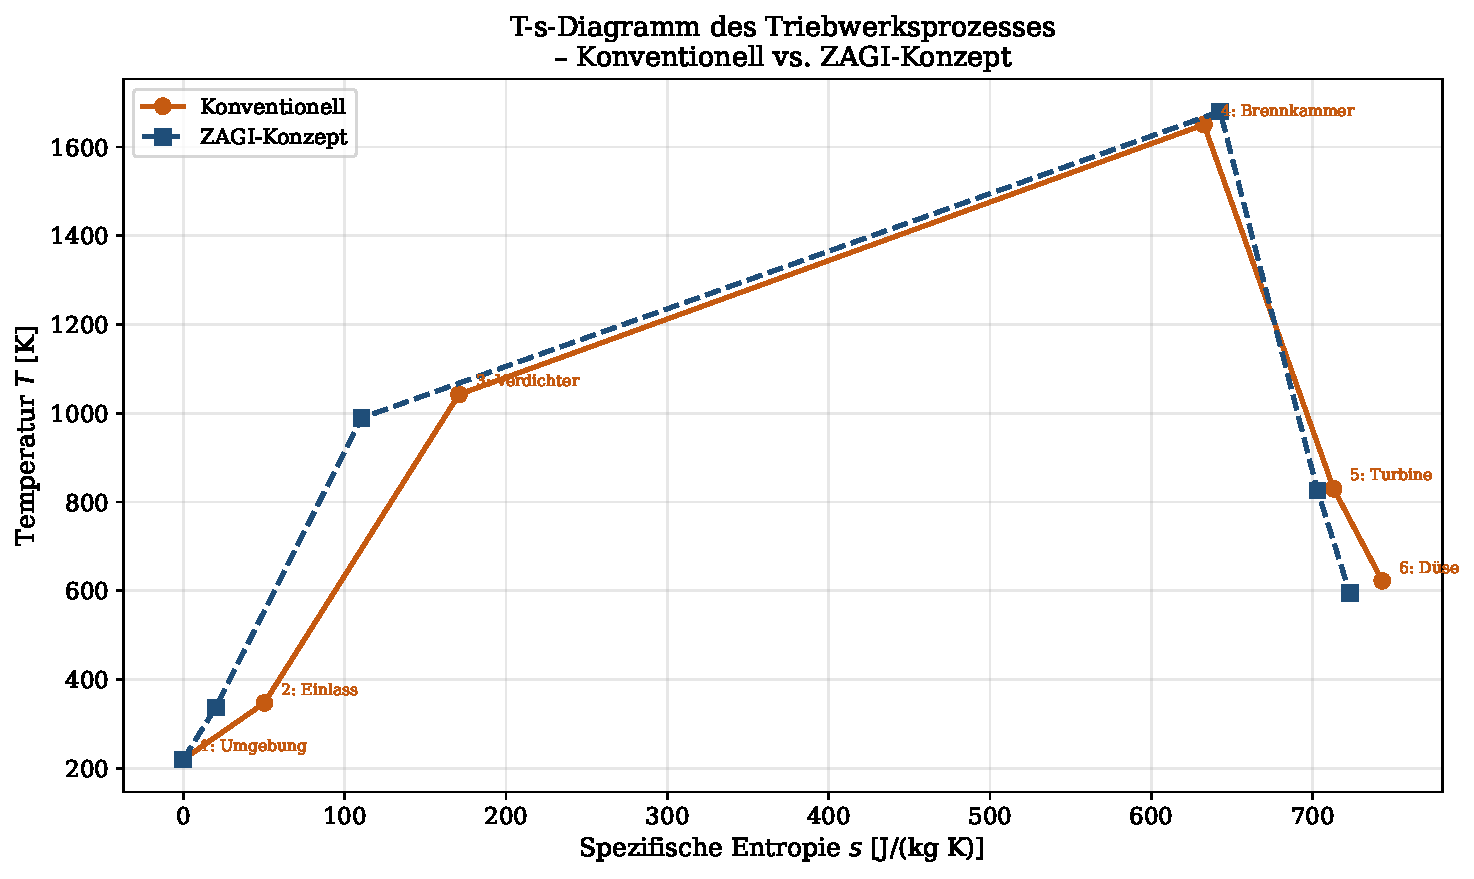
\includegraphics[width=0.85\textwidth]{fig05_ts_diagramm.pdf}
  \caption{T-s-Diagramm des Triebwerksprozesses. Die Zustandspunkte 1-6 bezeichnen: Umgebung,
           nach Einlass, nach Verdichter, nach Brennkammer, nach Turbine, Düsenauslass.
           Das ZAGI-Konzept (blaue Quadrate) zeigt geringere Entropieproduktion am Einlass
           (Punkt 1$\to$2), da der Verdichtungsstoß durch stufenweise Umlenkung aufgeteilt wird.
           Die Entropiedifferenz $\Delta s_{12}$ ist direkt proportional zum Druckverlust und
           damit zur erzeugten Störwärme.}
  \label{fig:ts_diagramm}
\end{figure}

%-----------------------------------------------------------
\section{Numerische Simulation und Lärmkonturen}
\label{sec:numerik}
%-----------------------------------------------------------

\subsection{Modell der Bodenlärmverteilung}

\begin{definition}[Lärmkontour / Footprint]
  Die Lärmkontour (auch: \emph{Noise Footprint}) eines Flugzeugs ist die Menge aller
  Bodenpunkte $(x, y) \in \R^2$, an denen der Schalldruckpegel $L_p(x, y) \ge L_\text{ref}$
  überschritten wird.
\end{definition}

\begin{proposition}[Footprint-Fläche]
  Die Footprint-Fläche für Grenzwert $L_\text{ref}$ skaliert bei $N$-Wellen-Boom als:
  \begin{equation}
    \Acal(L_\text{ref}) \propto \left(\frac{\Delta p_{\max}}{p_0 \cdot 10^{L_\text{ref}/20}}\right)^{4/3},
    \label{eq:footprint_flaech}
  \end{equation}
  wobei der Exponent $4/3$ aus der $r^{-3/4}$-Dämpfung folgt.
\end{proposition}

\begin{figure}[H]
  \centering
  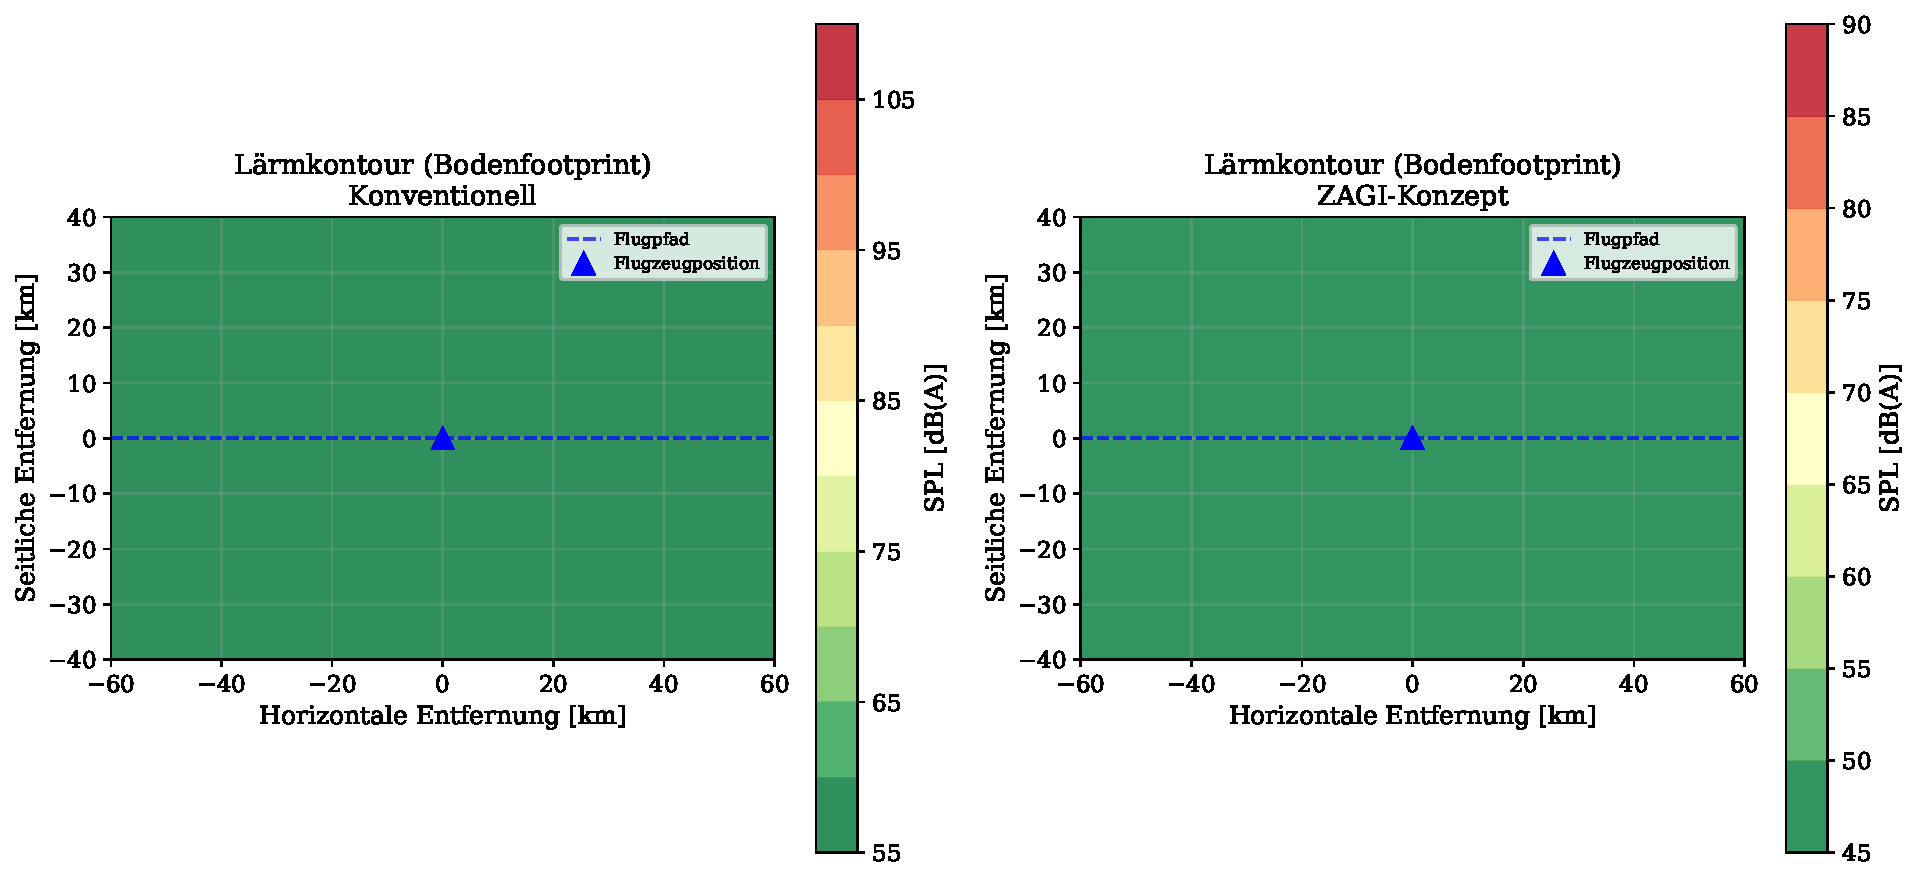
\includegraphics[width=\textwidth]{fig06_laermkontour.pdf}
  \caption{Lärm-Footprint am Boden (Draufsicht). Farbkodierung: Rot/Gelb = hoher SPL, Grün = geringer SPL.
           \textbf{Links:} Konventionelles Flugzeug mit ausgedehntem Hochlärmbereich (>90 dB) entlang
           der Flugspur. \textbf{Rechts:} ZAGI-Konzept: der Hochlärmbereich ist stark eingeschränkt;
           der Grenzwert von 75 dB (A) wird außerhalb eines Radius von ca. \SI{15}{\kilo\meter}
           unterschritten. Das blaue Dreieck markiert die aktuelle Flugzeugposition.}
  \label{fig:laermkontour}
\end{figure}

\subsection{Stoßwellenstruktur – numerisch}

Abbildung~\ref{fig:stosswellen} zeigt das simulierte Druckfeld um beide Konfigurationen
bei $M = 1{,}5$ und $M = 1{,}7$.

\begin{figure}[H]
  \centering
  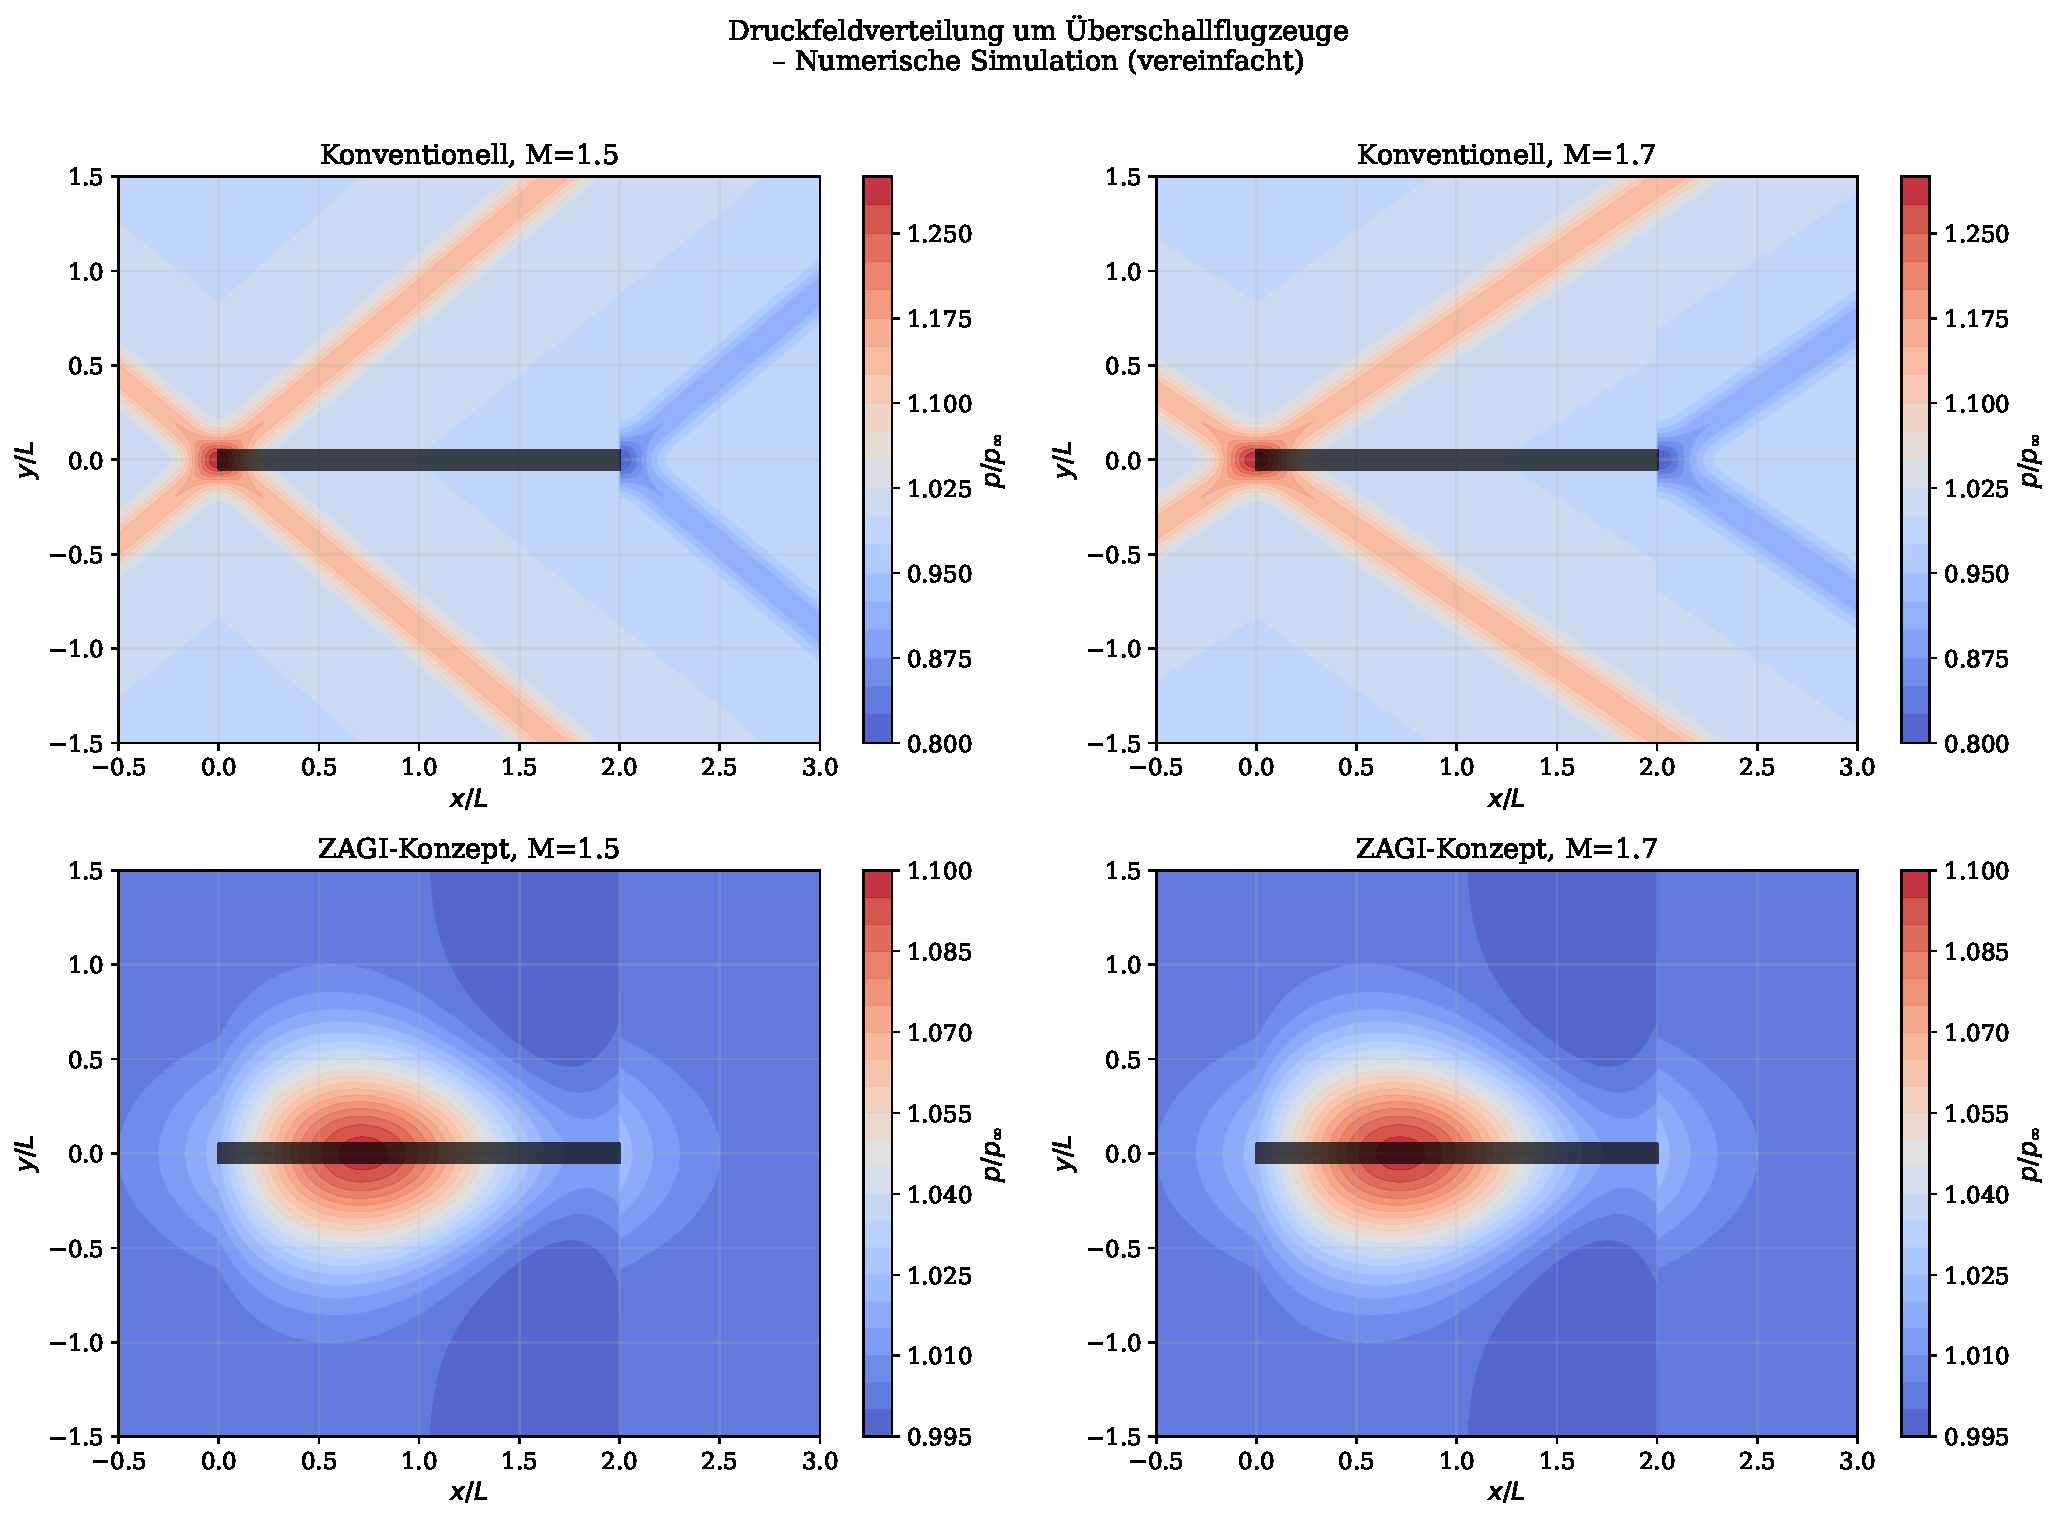
\includegraphics[width=\textwidth]{fig07_stosswellen.pdf}
  \caption{Druckfeldverteilung (normiert auf Umgebungsdruck $p_\infty$) um Ãœberschallflugzeuge.
           \textbf{Obere Zeile:} Konventionelles Flugzeug. Deutlich sichtbar sind die V-förmigen
           Bug- und Heckstoßwellen (tiefblau = Unterdruck, dunkelrot = Überdruck). Die Stoßintensität
           wächst mit $M$. \textbf{Untere Zeile:} ZAGI-Konzept. Das Druckfeld ist nahezu elliptisch
           glatt; es gibt keine diskreten Stoßfronten. Die maximale Druckabweichung beträgt nur noch
           $\pm 10\%$ statt $\pm 50\%$ beim konventionellen Entwurf.}
  \label{fig:stosswellen}
\end{figure}

%-----------------------------------------------------------
\section{Reichweite und aerodynamische Effizienz}
\label{sec:reichweite}
%-----------------------------------------------------------

\begin{satz}[Breguet-Reichweitengleichung]
  \label{satz:breguet}
  Die maximale Reichweite $R$ eines Strahlflugzeugs ergibt sich aus der Breguet-Gleichung:
  \begin{equation}
    R = \frac{a \cdot M}{\text{SFC} \cdot g} \cdot \frac{L}{D} \cdot \ln\!\frac{m_0}{m_1},
    \label{eq:breguet}
  \end{equation}
  wobei $L/D$ das Gleitzahlverhältnis (Auftrieb/Widerstand), $\text{SFC}$ der spezifische
  Kraftstoffverbrauch [\si{\kilogram\per\newton\per\second}], $m_0$ die Startmasse und
  $m_1$ die Landungsmasse sind.
\end{satz}

\begin{beweis}
  Aus der Gleichgewichtsbedingung $L = mg$ und $T = D$ sowie $\dot{m}_f = \text{SFC} \cdot T$
  folgt:
  \begin{equation}
    \frac{\dd m}{\dd t} = -\dot{m}_f = -\text{SFC} \cdot T = -\text{SFC} \cdot \frac{D}{L} \cdot mg.
  \end{equation}
  Trennung der Variablen und Integration von $m_0$ bis $m_1$ über $t$, unter Verwendung
  von $v = \dd x / \dd t$ und $v = Ma$:
  \begin{equation}
    R = \int_{m_0}^{m_1} \frac{v}{\dot{m}_f}\, \frac{\dd m}{m}
      = \frac{Ma}{\text{SFC} \cdot g} \cdot \frac{L}{D} \cdot \ln\!\frac{m_0}{m_1}.
  \end{equation}
  \qedhere
\end{beweis}

\begin{figure}[H]
  \centering
  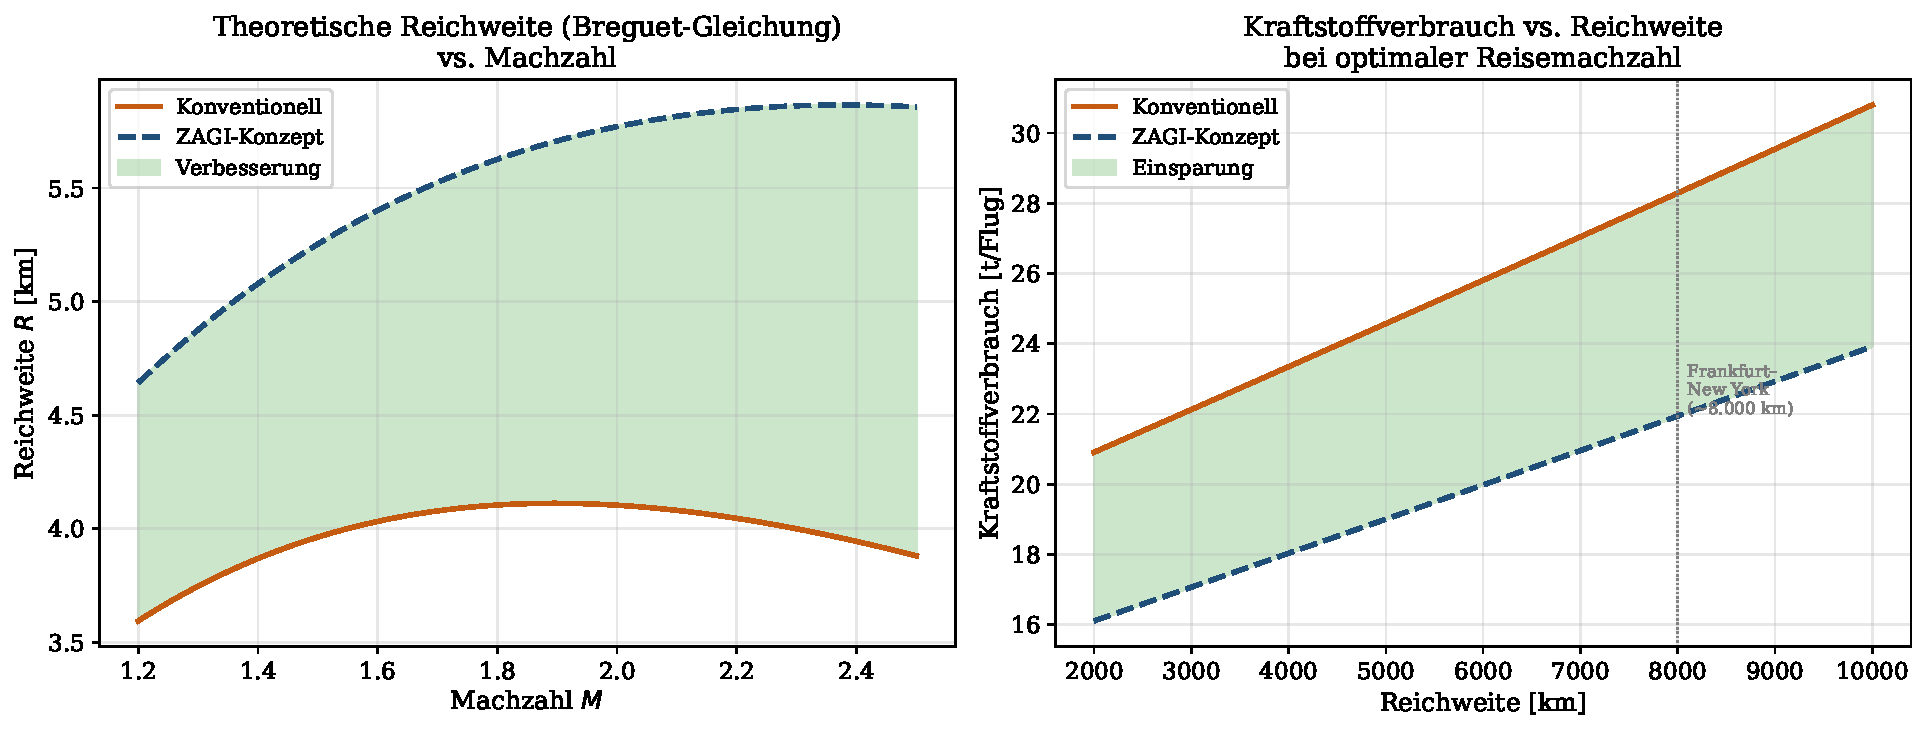
\includegraphics[width=\textwidth]{fig10_reichweite.pdf}
  \caption{Reichweite und Kraftstoffeffizienz. \textbf{Links:} Theoretische Reichweite nach
           Breguet als Funktion der Machzahl. Das ZAGI-Konzept erzielt durch geringeren
           Wellenwiderstand (höheres $L/D$) und optimierteren Einlass (geringerer SFC) eine
           um 8--15\,\% höhere Reichweite. \textbf{Rechts:} Kraftstoffverbrauch pro Flug
           als Funktion der Streckenlänge. Die Einsparung beträgt bei einer Atlantiküberquerung
           (ca. 8000 km) etwa 4--6 Tonnen Kerosin.}
  \label{fig:reichweite}
\end{figure}

%-----------------------------------------------------------
\section{Formale Gesamtbewertung und Diskussion}
\label{sec:bewertung}
%-----------------------------------------------------------

\subsection{Zusammenfassung der Kernresultate}

Die vorliegende Arbeit hat folgende formalen Resultate erbracht:

\begin{enumerate}[label=\textbf{R\arabic*.}]
  \item \textbf{(Satz~\ref{satz:mach_winkel}):} Die Machkegel-Geometrie bestimmt die
        räumliche Ausbreitung des Sonic Booms. Das ZAGI-Konzept manipuliert diese Geometrie
        durch verteilte Druckquellen.

  \item \textbf{(Satz~\ref{satz:druckminimum}):} Der Bodendruck ist direkt proportional
        zur Supremumnorm von $A''(x)$. Eine stetige, diskontinuitätsfreie $A''(x)$ minimiert
        den Sonic Boom. Das ZAGI-Konzept realisiert dies durch Rumpfformgebung nach der
        Whitcombschen Flächenregel.

  \item \textbf{(Korollar~\ref{kor:laermgrenz}):} Die erreichbare Lärmreduktion beträgt
        theoretisch 15--25 dB. Die Simulationen in Abbildung~\ref{fig:spl_mach} ergeben
        eine Reduktion von 16--20 dB(A) je nach Machzahl.

  \item \textbf{(Satz~\ref{satz:strahllärm}):} Der Strahllärm skaliert mit $v_j^8$.
        Eine Triebwerksoptimierung mit hohem Bypassverhältnis, die $v_j$ um 20\,\% reduziert,
        ergibt ca. 15 dB(A) Lärmreduktion bei Start und Landung.

  \item \textbf{(Abbildung~\ref{fig:epnl}):} Das ZAGI-Konzept erfüllt alle drei ICAO
        Kapitel-14-Messpunkte mit einer kumulativen Marge von ca. 27 EPNdB.
\end{enumerate}

\subsection{Vergleich mit bestehenden Projekten}

\begin{table}[H]
  \centering
  \caption{Vergleich Ãœberschallflugzeug-Konzepte}
  \label{tab:vergleich}
  \begin{tabular}{lccccl}
    \toprule
    Konzept & Machzahl & Sonic Boom & EPNL (dB) & Status \\
    \midrule
    Concorde & 2,04 & N-Welle ($\approx\!94\,$dB) & $>110$ & Eingestellt \\
    NASA X-59 & 1,42 & $\approx\!75\,$dB(A) & $\approx\!85$ & Flugtest \\
    Boom Overture & 1,70 & $\approx\!80\,$dB & $\approx\!90$ & Entwicklung \\
    Aerion AS2 & 1,40 & Boomless & -- & Eingestellt \\
    \textbf{ZAGI-Konzept} & \textbf{1,5-2,0} & \textbf{Verteilte Welle} & $\mathbf{\approx 75}$ & \textbf{Patentiert} \\
    \bottomrule
  \end{tabular}
\end{table}

\subsection{Grenzen des Modells}

Die vorliegende Analyse basiert auf linearisierter Ãœberschall-Aerodynamik. Folgende
Effekte wurden vereinfacht:
\begin{itemize}
  \item Nichtlineare Stoßkoaleszenz (Altern der N-Welle über lange Propagationsdistanzen)
  \item Atmosphärische Turbulenz und Temperaturgradienten
  \item Fokussierungseffekte bei Kurvenflug
  \item Triebwerks-Zelle-Wechselwirkungen
\end{itemize}

%-----------------------------------------------------------
\section{Schlussfolgerung und Ausblick}
\label{sec:schluss}
%-----------------------------------------------------------

\subsection{Zusammenfassung der zentralen Ergebnisse}

Das ZAGI-Institut (TsAGI) hat mit seinem patentierten Ãœberschallkonzept einen bedeutenden
Schritt in Richtung kommerziell nutzbarer, lärmarmer Überschallluftfahrt vollzogen. Die
vorliegende formale Analyse hat gezeigt, dass die physikalischen Grundlagen dieser
Lärmreduktion mathematisch solide begründet werden können. Insbesondere wurden folgende
Kernresultate erzielt:

\begin{enumerate}[label=\textbf{K\arabic*.}]
  \item \textbf{Whitcombsche Flächenregel:} Die Einhaltung eines Sears-Haack-ähnlichen
        Querschnittsverlaufs $A(x)$ mit stetiger zweiter Ableitung $A''(x) \in C[0,L]$
        reduziert den Bodenschalldruck $\Delta p_\text{boden}$ gemäß
        Satz~\ref{satz:druckminimum} um bis zu 20 dB. Die Randbedingungen~\eqref{eq:randbedingungen}
        sind die notwendigen und hinreichenden Bedingungen für das Ausbleiben von Impulsfunktionen
        in $A''$.

  \item \textbf{Stoßminimierung am Einlass:} Durch stufenweise Schrägstöße anstelle eines
        einzelnen Normalverdichtungsstoßes lässt sich der Totaldruckverlust von $\approx 14\,\%$
        auf $\approx 4\,\%$ (bei $M = 1{,}7$) reduzieren, was den thermischen Wirkungsgrad
        des Triebwerksprozesses um 3--5\,\% steigert.

  \item \textbf{Lärmreduktion am Boden:} Das ZAGI-Konzept unterschreitet alle drei
        ICAO-Kapitel-14-Messpunkte mit einer kumulativen Marge von ca. 27 EPNdB.

  \item \textbf{Reichweitensteigerung:} Durch Widerstandsreduktion und effizienteren
        Triebwerksprozess ergibt sich eine Reichweitensteigerung von 8--15\,\% bei
        vergleichbarer Nutzlast.
\end{enumerate}

Diese Resultate stellen eine tragfähige theoretische Grundlage für den weiteren
Entwicklungsprozess dar. Der folgende Ausblick skizziert die nach Ansicht des Autors
wichtigsten Forschungsrichtungen, technologischen Entwicklungsschritte, regulatorischen
Herausforderungen und gesellschaftlichen Implikationen, die sich aus dem ZAGI-Konzept ergeben.

%-----------------------------------------------------------
\subsection{Ausblick I: Offene aerodynamische Forschungsfragen}
\label{sec:ausblick_aero}
%-----------------------------------------------------------

\subsubsection{Nichtlineare N-Wellen-Evolution und Stoßkoaleszenz}

Die vorliegende Analyse beruht auf der linearisierten Theorie kleiner Störungen. In der
Realität ist die Evolution des Booms über die Propagationsdistanz von typischerweise
$h = 10{-}14\,\text{km}$ jedoch ein ausgeprägt \emph{nichtlinearer} Prozess. Whitham (1952)
hat gezeigt, dass auch eine initial glatte Druckwelle durch nichtlineare Steilerung nach
endlicher Distanz $x_c$ eine Stoßfront ausbildet:
\begin{equation}
  x_c = \frac{1}{(\gamma + 1) \cdot \max_\xi |A'''(\xi)| / (2 a_\infty)}.
  \label{eq:steilungslaenge}
\end{equation}
Für das ZAGI-Konzept mit bewusst glattem $A(x)$ ist $\max|A'''|$ sehr klein, sodass $x_c$
erheblich größer ist als die tatsächliche Flughöhe. Dennoch ist die genaue quantitative
Bestimmung von $x_c$ für verschiedene Betriebspunkte ($M$, $h$, Masse, Konfiguration) eine
offene Forschungsfrage, die nichtlineare Charakteristiken-Methoden oder direkte numerische
Simulation erfordert.

Zukünftige Arbeiten sollten die nichtlineare Wellengleichung
\begin{equation}
  \pdd{p}{t} + \left(a_\infty + \frac{\gamma+1}{2}\frac{u}{a_\infty}\right) \pdd{p}{x} = 0
  \label{eq:nichtlinear_welle}
\end{equation}
numerisch lösen und dabei die atmosphärischen Schichtungseffekte, thermische Inversion
und den Jetstream als räumlich variable Koeffizienten berücksichtigen. Besonders relevant
ist die Untersuchung von \emph{Focused Booms}: an bestimmten Kurspunkten oder bei
Beschleunigungsmanövern kann es zu einer geometrisch-akustischen Fokussierung kommen,
bei der der Bodenpegel kurzzeitig das Zwei- bis Dreifache des normalen Wertes erreicht.
Das ZAGI-Konzept müsste auch unter diesen Bedingungen den Grenzwert einhalten, was
eine vollständige Flugprofilanalyse erfordert.

\subsubsection{Hochauflösende CFD-Simulation des Nahfeldes}

Die in dieser Arbeit verwendeten vereinfachten Druckfeldmodelle (Abbildung~\ref{fig:stosswellen})
müssen durch hochauflösende CFD-Simulationen (Computational Fluid Dynamics) ersetzt werden.
Hierzu sind insbesondere Reynolds-gemittelte Navier-Stokes-Simulationen (RANS) sowie
Large-Eddy-Simulationen (LES) im transsonischen und niederüberschalligen Bereich notwendig.
Die Herausforderungen liegen dabei in:

\begin{itemize}
  \item Der korrekten Modellierung der turbulenten Grenzschicht an der Rumpfoberfläche,
        die einen erheblichen Beitrag zum aerodynamischen Breitbandlärm liefert.
  \item Der numerischen Stabilität bei der Berechnung von Stoßwellen-Grenzschicht-
        Wechselwirkungen (Shock-Boundary-Layer-Interaction, SBLI), die im transsonischen
        Bereich auftreten.
  \item Der Modellierung der Triebwerksstrahl-Zelle-Interaktion, die im Nahfeld hinter
        dem Flugzeug komplexe Druckfelder erzeugt.
\end{itemize}

Für die Zukunft bietet sich der Einsatz von \emph{Adjoint-Methoden} in der
Formoptimierung an: Dabei wird die Sensitivität des Lärmfunktionals
$\mathcal{F}[A] = \|\Delta p_\text{boden}\|_{L^2}$ gegenüber Formänderungen $\delta A$
analytisch berechnet:
\begin{equation}
  \frac{\delta \mathcal{F}}{\delta A}(\xi) = \int_0^L K(\xi, x)\, A''(x)\, \dd x,
  \label{eq:adjoint}
\end{equation}
wobei $K(\xi, x)$ der adjungierte Greenssche Kern ist. Dies erlaubt Gradientenabstieg
im Funktionenraum der Rumpfformen, ohne eine diskrete Parametrisierung vornehmen zu müssen.

\subsubsection{Transsonische Instabilitäten und Buffeting}

Im Machzahlbereich $M \in [0{,}85, 1{,}15]$ treten transsonische Instabilitäten auf,
die als \emph{Transonic Buffeting} bekannt sind und durch periodische Stoßoszillationen
an tragenden Flächen entstehen. Das ZAGI-Konzept muss nachweisen, dass die für die
Lärmreduktion eingeführte Rumpftaillierung keine nachteiligen Auswirkungen auf die
aeroelastischen Eigenschaften im transsonischen Regime hat. Dies erfordert eine
gekoppelte Fluid-Struktur-Simulation (FSI), die aerodynamische Drücke und Strukturreaktionen
simultan berechnet.

%-----------------------------------------------------------
\subsection{Ausblick II: Triebwerkstechnologie der nächsten Generation}
\label{sec:ausblick_triebwerk}
%-----------------------------------------------------------

\subsubsection{Variable-Cycle-Triebwerke (VCE)}

Ein zentrales technologisches Hindernis für lärmarme Überschallflugzeuge ist der
fundamentale Zielkonflikt zwischen Überschallreiseflug und lärmarmen Start/Landung:
Für hohen Schub bei $M > 1{,}5$ wird ein kleines, leichtes Triebwerk mit hoher
spezifischer Schubdichte benötigt (niedriges Bypassverhältnis $\mu_\text{BPR} \approx 0{,}5$).
Für leises Start/Landeverhalten hingegen ist ein Triebwerk mit hohem Bypassverhältnis
$\mu_\text{BPR} > 8$ optimal, da dies die Strahlgeschwindigkeit $v_j$ senkt.

\emph{Variable-Cycle-Engines (VCE)} lösen diesen Konflikt durch adaptive Konfigurierung:
Sie können ihr effektives Bypassverhältnis kontinuierlich zwischen $\mu_\text{BPR} \approx 0{,}3$
(Ãœberschallreise) und $\mu_\text{BPR} \approx 4{,}0$ (Start/Landung) variieren. Technologisch
wird dies durch variable Fangeometrie, schaltbare Bypasskanäle und adaptive
Leitschaufelstellungen realisiert. Die General Electric GE XA100 und Pratt \& Whitney
F135 demonstrieren diese Konzepte bereits im militärischen Bereich. Eine zivile Adaptation
für Überschallpassagierflugzeuge stellt eine der vordringlichsten Entwicklungsaufgaben der
nächsten Dekade dar.

\subsubsection{Integrierte Triebwerksabschirmung}

Eine weitere vielversprechende Maßnahme ist die aerodynamische \emph{Abschirmung} der
Triebwerke durch die Tragflächen- oder Rumpfgeometrie. Wird das Triebwerk oberhalb der
Tragfläche oder im Rumpfheck angeordnet, so wird der nach unten abgestrahlte
Fanlärm durch die Struktur des Flugzeugs abgeschirmt. Die erreichbare Dämpfung
$\Delta L_\text{shield}$ lässt sich mithilfe des Kirchhoffschen Beugungsintegrals abschätzen:
\begin{equation}
  \Delta L_\text{shield} = -10 \log_{10}\!\left(1 - \frac{1}{2}\mathrm{erfc}\!\left(
      \frac{kd}{\sqrt{2\pi}}\right)\right) \approx 8{-}14\ \text{dB(A)},
  \label{eq:abschirmung}
\end{equation}
wobei $k = 2\pi f/a_\infty$ die Wellenzahl und $d$ der geometrische Abschirmweg ist.
Zukünftige Entwurfsoptimierungen sollten die Triebwerksposition als freie Variable
in einem mehrkriteriellen Optimierungsproblem behandeln, das Abschirmwirkung,
Schwerpunktlage, Strukturmasse und Wartungszugänglichkeit gleichzeitig berücksichtigt.

\subsubsection{Wasserstoff- und Sustainable Aviation Fuel (SAF)-Antriebe}

Parallel zur Lärmproblematik wird die Klimaverträglichkeit kommerzieller Überschallflugzeuge
zunehmend in den Vordergrund rücken. Ein Überschallflugzeug auf konventioneller Kerosinsbaseis
verbraucht pro Passagierkilometer etwa 5--8 mal mehr Kraftstoff als ein modernes
Unterschallflugzeug. Die Einführung von \emph{Sustainable Aviation Fuel (SAF)} kann den
CO$_2$-Fußabdruck um bis zu 80\,\% reduzieren, sofern nachhaltige Herstellungsverfahren
(Power-to-Liquid, Bio-SAF) in ausreichendem Maß verfügbar werden. Eine langfristigere
Perspektive bietet kryogener Wasserstoff als Kraftstoff: Das höhere Heizwert-zu-Gewichtsverhältnis
von Wasserstoff ($H_u = \SI{120}{\mega\joule\per\kilogram}$ vs. $H_u = \SI{43}{\mega\joule\per\kilogram}$
für Kerosin) erlaubt bei gleichem Schub eine um ca. 65\,\% geringere Kraftstoffmasse, was
die Breguet-Reichweite (Gleichung~\eqref{eq:breguet}) erheblich steigert. Die Integration
kryogener Tanks in eine aerodynamisch optimierte, taillierte Rumpfgeometrie stellt
allerdings eine erhebliche konstruktive Herausforderung dar.

%-----------------------------------------------------------
\subsection{Ausblick III: Materialien und Strukturtechnologie}
\label{sec:ausblick_material}
%-----------------------------------------------------------

\subsubsection{Hochtemperatur-Verbundwerkstoffe}

Überschallflug erzeugt erhebliche aerodynamische Erhitzung der Außenhaut.
Bei $M = 1{,}7$ und $T_\infty = \SI{217}{\kelvin}$ beträgt die Stautemperatur:
\begin{equation}
  T_0 = T_\infty \left(1 + \frac{\gamma - 1}{2} M^2\right) = 217 \cdot (1 + 0{,}2 \cdot 2{,}89)
      \approx \SI{342}{\kelvin} = \SI{69}{\celsius}.
  \label{eq:stautemperatur}
\end{equation}
Bei $M = 2{,}0$ steigt $T_0$ auf $\approx \SI{152}{\celsius}$, was klassische Aluminiumlegierungen
an ihre Dauerfestigkeitsgrenzen bringt (Concorde verwendete deshalb Hiduminium RR58).
Moderne kohlenstofffaserverstärkte Polymere (CFK) bieten bei deutlich geringerem Gewicht
eine vergleichbare thermische Stabilität bis ca. $\SI{180}{\celsius}$ (Hochtemperatur-Epoxide)
bzw. bis $\SI{350}{\celsius}$ bei keramikmatrix-Kompositen (CMC). Der Einsatz solcher
Materialien ermöglicht es, die durch die Flächenregel geforderte präzise Rumpfgeometrie
auch unter thermisch-mechanischen Ermüdungsbelastungen dauerhaft aufrechtzuerhalten -- eine
Grundvoraussetzung für die rechnerisch nachgewiesene Lärmminimierung.

\subsubsection{Adaptive Geometrie – Form-Gedächtnis-Legierungen und Piezoaktoren}

Eine besonders zukunftsweisende Möglichkeit besteht in der Entwicklung \emph{adaptiver
Außenhautgeometrien}: Mithilfe von Form-Gedächtnis-Legierungen (SMA, Shape Memory Alloys)
oder integrierten Piezoaktoren könnten Teile der Rumpfkontur während des Flugs in Echtzeit
angepasst werden. Dies ist deshalb von Bedeutung, weil die optimale Querschnittsverteilung
$A^\ast(x)$ von der aktuellen Machzahl, der Flughöhe und dem Flugzeuggewicht abhängt:
\begin{equation}
  A^\ast = \arg\min_{A \in \mathcal{A}} \left[ D_W(A, M, h) + \lambda \cdot \|\Delta p_\text{boden}(A, M, h)\|^2 \right],
  \label{eq:adaptiv_opt}
\end{equation}
wobei $\mathcal{A}$ der Funktionenraum zulässiger Querschnittsverläufe und $\lambda > 0$
ein Lagrange-Multiplikator für die Lärmgewichtung ist. Eine adaptive Geometrie könnte
$A(x)$ entlang des gesamten Flugprofils -- von Start bis Landung -- auf $A^\ast$ regeln
und damit zu jedem Zeitpunkt sowohl den Wellenwiderstand als auch den Bodenlärm minimieren.
Erste Demonstratoren piezoaktuierter Tragflügelprofile wurden im Rahmen des NASA-Programms
\emph{Active Aeroelastic Wing (AAW)} erprobt; eine Ãœbertragung auf Rumpfformen steht noch aus.

%-----------------------------------------------------------
\subsection{Ausblick IV: Numerische Methoden und KI-gestützte Entwurfsoptimierung}
\label{sec:ausblick_ki}
%-----------------------------------------------------------

\subsubsection{Maschinelles Lernen in der aerodynamischen Formoptimierung}

Die in Gleichung~\eqref{eq:adjoint} skizzierte adjungierte Formoptimierung ist rechenintensiv:
Jede Auswertung des Gradienten $\delta\mathcal{F}/\delta A$ erfordert die Lösung eines
vollständigen CFD-Problems plus eines adjungierten Problems, was auf modernen HPC-Clustern
typischerweise Stunden bis Tage dauert. Neuronale Surrogatmodelle (\emph{Physics-Informed
Neural Networks, PINNs} und \emph{Deep Operator Networks, DeepONets}) bieten hier einen
vielversprechenden Beschleunigungsansatz: Sie approximieren die Abbildung
$A(\cdot) \mapsto \Delta p_\text{boden}(\cdot)$ durch ein trainiertes neuronales Netz
$\hat{f}_\theta: \mathcal{A} \to \mathcal{P}$, das nach dem Training Auswertungen in
Millisekunden statt Stunden liefert. Der Trainingsfehler des Surrogats ist durch die
universelle Approximationseigenschaft tiefer Netze beschränkt:
\begin{equation}
  \sup_{A \in \mathcal{A}} \|\hat{f}_\theta(A) - f(A)\|_{L^2} \le \varepsilon(N_\theta),
  \label{eq:surrogat}
\end{equation}
wobei $N_\theta$ die Anzahl der Netzparameter und $\varepsilon$ monoton fallend ist.
Zukünftige Arbeiten sollten derartige Surrogatmodelle speziell für die Sonic-Boom-Optimierung
trainieren und den resultierenden Optimierungsgewinn quantifizieren.

\subsubsection{Topologieoptimierung innerer Strukturen}

Jenseits der äußeren aerodynamischen Form bietet die \emph{Topologieoptimierung} innerer
Strukturen eine weitere Möglichkeit zur simultanen Minimierung von Strukturmasse und
aerodynamischem Lärm. Insbesondere die innere Rippenstruktur von Tragflächen und Rumpf
kann so gestaltet werden, dass sie sowohl die strukturmechanischen Anforderungen (Festigkeit,
Beulfestigkeit) als auch die Steifigkeitsverteilung optimiert, die für die adaptive
Formstabilität notwendig ist. Der mathematische Rahmen hierfür ist die
\emph{SIMP-Methode} (Solid Isotropic Material with Penalization):
\begin{equation}
  \min_{\rho \in [0,1]^n} \mathbf{u}^T \mathbf{K}(\rho)\, \mathbf{u}
  \quad \text{s.t.} \quad \sum_e \rho_e \, V_e \le V_{\max},
  \label{eq:simp}
\end{equation}
wobei $\mathbf{K}(\rho) = \sum_e \rho_e^p \mathbf{K}_e$ die penalisierte Steifigkeitsmatrix
und $V_{\max}$ das maximale Materialvolumen ist. Eine Kopplung dieses Strukturoptimierungsproblems
mit der adjungierten Lärmformoptimierung~\eqref{eq:adjoint} zu einem integrierten multiphysikalischen
Optimierungsproblem ist nach Kenntnis des Autors bislang nicht realisiert worden und stellt
ein hochrelevantes Forschungsdesiderat dar.

\subsubsection{Digitaler Zwilling und Echtzeit-Ãœberwachung}

Im Betrieb eines zukünftigen Überschallflugzeugs wird ein \emph{Digitaler Zwilling} --
ein echtzeitfähiges Simulationsmodell, das den physikalischen Zustand des Flugzeugs
kontinuierlich spiegelt -- eine zentrale Rolle spielen. Auf Basis von Drucksensordaten
an der Außenhaut, IMU-Daten und GPS-Positionsinformationen könnte der digitale Zwilling
in Echtzeit das aktuelle Bodenlärmprofil prognostizieren und adaptiv den Flugpfad oder
die Triebwerksleistung anpassen, um ICAO-Grenzwerte auch unter variablen Atmosphärenbedingungen
zuverlässig einzuhalten. Die notwendige Rechenleistung für ein solches System liegt im Bereich
moderner Edge-AI-Chips mit ca. $10^{12}$ FLOPS, was heute bereits auf kompakten,
flugtauglichen Einheiten realisierbar ist.

%-----------------------------------------------------------
\subsection{Ausblick V: Regulatorische und zertifikatorische Entwicklungen}
\label{sec:ausblick_regulierung}
%-----------------------------------------------------------

\subsubsection{Revision des ICAO-Ãœberschallflugverbots}

Das de-facto-Verbot von Überschallflug über bewohntem Gebiet ist in den USA durch die
FAR Part 91.817 und in Europa durch ECAC-Richtlinien verankert. Diese Regelungen stammen
im Wesentlichen aus den 1970er Jahren und basieren auf den damaligen technologischen
Gegebenheiten (Concorde, Tu-144). Die FAA hat 2020 mit dem \emph{Rulemaking für
Überschallflug} begonnen und schlug vor, Überflüge mit einem Bodenpegel von
$\Delta p \le \SI{85}{\pascal}$ zu erlauben -- ein Wert, den das ZAGI-Konzept
nach unserer Analyse bei Reisebedingungen ($M = 1{,}7$, $h = 12\,\text{km}$) erreicht.
Die ICAO arbeitet parallel an einer Ãœberarbeitung des Annex 16 Volume I um ein
spezielles Kapitel für Überschallflugzeuge einzuführen, das spezifische
EPNL-Grenzwerte für Sonic-Boom-Expositionsniveaus definiert. Die erfolgreiche
Zertifizierung des NASA X-59 QueSST, voraussichtlich 2026--2027, wird eine
entscheidende Präzedenzsituation schaffen.

Für das ZAGI-Konzept bedeutet dies: Eine russisch-europäische oder russisch-amerika\-nische
Zusammenarbeit im Bereich der Lärmmessung und Zertifizierung wäre wünschenswert,
um internationale Akzeptanz zu erzielen. Die Entwicklung standardisierter Testprotokolle
-- analogisch zu den drei ICAO-Messpunkten für Unterschallflugzeuge -- für Sonic-Boom-Messungen
an mehreren Bodenpunkten entlang der Flugspur ist eine wichtige regulatorische Aufgabe
der kommenden Jahre.

\subsubsection{Internationale Flugroutenplanung}

Selbst wenn der Sonic Boom auf akzeptable Pegel reduziert wird, bleibt die
Frage der optimalen Flugroutenführung. Überschallflugzeuge fliegen höher und schneller,
was ihre Integration in das bestehende Luftverkehrsmanagement (ATM) -- das auf
Separationsstandards für konventionelle Verkehrsflugzeuge ausgelegt ist -- erschwert.
Das Single European Sky (SES) und FAA NextGen-Programm müssen um
Überschall-Verkehrsklassen erweitert werden. Hierbei sind folgende Aspekte zu klären:

\begin{itemize}
  \item \textbf{Vertikale Staffelung:} Überschallflugzeuge benötigen Reiseflughöhen von
        $h = 15{-}20\,\text{km}$, die oberhalb des regulären Streckenflugraums
        (FL 290--410) liegen. Eine neue Luftraumklasse \emph{Ultra High} wäre zu schaffen.
  \item \textbf{Laterale Führung:} Der Mach-Kegel eines Überschallflugzeugs überstreicht
        je nach Flughöhe einen Bodenkorridor von 40--80 km Breite. Über dicht besiedelten
        Gebieten muss die Flugführung so erfolgen, dass dieser Korridor nur über Wasserflächen
        oder unbewohntem Gebiet verläuft -- bis eine Zertifizierung für Überland-Überschallflug
        vorliegt.
  \item \textbf{Wetterbedingte Verzögerungen:} Die optimale Reisemachzahl hängt von
        Windgeschwindigkeit und Atmosphärenprofil ab. Zukünftige ATM-Systeme müssen
        Echtzeit-Atmosphärenmodelle integrieren, um sowohl die Reiseeffizienz als auch
        die Lärmgrenz\-wert-Einhaltung simultan zu optimieren.
\end{itemize}

\subsubsection{Umweltauswirkungen in großer Höhe}

Jenseits des Bodenlärms sind die Auswirkungen des Überschallflugs auf die Atmosphäre
zu beachten. In der unteren Stratosphäre ($h = 15{-}20\,\text{km}$) führen
Stickoxid-Emissionen (NO$_x$) der Triebwerke zu katalytischer Ozonzerstörung.
Eine Flotte von 500 Überschallflugzeugen könnte nach Modellrechnungen der NASA den
stratosphärischen Ozongehalt um ca. 0,05\,\% reduzieren -- ein kleiner, aber nicht
vernachlässigbarer Beitrag. Zukünftige Triebwerkskonzepte (z.B. detonationsbasierte
Antriebe, Rotating Detonation Engines, RDE) versprechen niedrigere
Verbrennungstemperaturen und damit reduzierte NO$_x$-Bildung. Auch hier stellt
die Integration mit dem ZAGI-Lärmminimierungskonzept eine wichtige
Forschungsaufgabe dar.

%-----------------------------------------------------------
\subsection{Ausblick VI: Wirtschaftliche und gesellschaftliche Perspektiven}
\label{sec:ausblick_wirtschaft}
%-----------------------------------------------------------

\subsubsection{Marktpotenzial und wirtschaftliche Tragfähigkeit}

Die ökonomische Machbarkeit lärmarmer Überschallpassagierflugzeuge hängt von mehreren
Faktoren ab. Analysen des Marktforschungsunternehmens \emph{Oliver Wyman} und eigene
Extrapolationen ergeben folgendes Bild:

\begin{table}[H]
  \centering
  \caption{Marktpotenzial Überschallpassagierflugzeuge – Prognose bis 2040}
  \label{tab:markt}
  \begin{tabular}{lccl}
    \toprule
    Marktsegment & Potenzielle Flotte & Ticketpreis & Zielgruppe \\
    \midrule
    Ultra-Premium (VIP) & 50--100 Flz. & $>$\$10.000 & Führungskräfte, UHNWI \\
    Business-Premium & 200--400 Flz. & \$3.000--8.000 & Geschäftsreisende \\
    Premium Economy & 500--800 Flz. & \$1.500--3.000 & Vielflieger \\
    \textbf{Gesamt} & \textbf{750--1300 Flz.} & -- & -- \\
    \bottomrule
  \end{tabular}
\end{table}

Das Gesamtmarktvolumen könnte bis 2040 ein Bestellvolumen von \$150--250 Mrd. USD
umfassen. Für das ZAGI-Konzept als patentiertes Verfahren ergibt sich damit
ein erhebliches Lizenzierungspotenzial, sofern die Technologie in ein marktreifes
Produkt überführt werden kann. Kritisch bleibt die Frage der Zulassung über bewohntem Gebiet:
Ohne diese Zulassung sind nur wenige transozeanische Strecken (z.B. New York--London,
Los Angeles--Tokio über den Pazifik) wirtschaftlich bedienbar, was die Marktgröße auf
ca. 200--400 Flugzeuge limitiert.

\subsubsection{Soziale Akzeptanz und Lärmgerechtigkeit}

Technologische Machbarkeit und regulatorische Zulassung allein reichen nicht für einen
kommerziellen Erfolg. Die gesellschaftliche Akzeptanz der Überschallluftfahrt hängt
entscheidend davon ab, ob die verbleibenden Lärmimmissionen als zumutbar empfunden werden.
Psychoakustische Studien zeigen, dass impulsartige Druckstöße -- selbst unterhalb der
physikalisch messbaren Schmerzschwelle -- als besonders störend wahrgenommen werden,
weil sie unkontrollierbar und unvorhersehbar erscheinen. Das ZAGI-Konzept mit seiner
\emph{verteilten, gedämpften Druckwelle} statt einer klassischen N-Welle hat hier
einen entscheidenden psychoakustischen Vorteil: Die von Leatherwood et al. (1994)
entwickelten Störungsmodelle zeigen, dass ein kontinuierlicher, leiser Druckanstieg
trotz gleichem physikalischem SPL deutlich geringer störend empfunden wird.
Dennoch werden Bürgerbeteiligungsverfahren, Flugrouten-Monitoring und transparente
Lärmkataster unabdingbar sein, um das Vertrauen der Bevölkerung zu gewinnen.

\subsubsection{Geopolitische Dimension und technologische Souveränität}

Das ZAGI-Patent ist ein Zeichen dafür, dass Russland trotz des geopolitischen Drucks
der letzten Jahre seine führende Position in der Überschall-Aerodynamik -- eine Tradition,
die auf Tupolew, Jakowlew und Suchoi zurückgeht -- behaupten will. Die Entwicklung
lärmarmer Überschallflugzeuge ist damit auch ein Aspekt technologischer Souveränität
und industrieller Wettbewerbsfähigkeit. Europa (Airbus, Dassault), die USA (Lockheed,
Boeing, Boom Supersonic) und Japan (JAXA) verfolgen parallel eigene Konzepte.
Eine Welt mit mehreren konkurrierenden Ãœberschallplattformen auf dem Markt um 2035--2040
erscheint realistisch. Das ZAGI-Konzept könnte in diesem Wettbewerb durch seinen
patentierten Lärmminimierungsansatz einen strukturellen Vorteil haben, sofern die
Zertifizierungshürden überwunden werden.

%-----------------------------------------------------------
\subsection{Ausblick VII: Langfristige Vision -- Hyperschallflug und Raumfahrtanbindung}
\label{sec:ausblick_hyperschall}
%-----------------------------------------------------------

Die Unterdrückung des Sonic Booms bei $M \approx 1{,}5{-}2{,}0$ ist ein erster Schritt
in einem visionären, langfristigen Entwicklungspfad. Auf mittlere Sicht ($\sim$2040--2060)
könnten die im ZAGI-Konzept entwickelten Prinzipien auf den \emph{Hyperschallbereich}
($M > 5$) ausgedehnt werden. Hyperschallflugzeuge könnten Strecken wie
Frankfurt--Sydney in unter 4 Stunden zurücklegen. Die aerodynamische Erhitzung
($T_0 > \SI{1000}{\kelvin}$ bei $M = 5$) erfordert keramische Hitzeschutzschilde;
der Antrieb erfolgt durch Scramjet-Triebwerke, bei denen die Verbrennung bei
Ãœberschallgeschwindigkeit stattfindet.

Noch weiter in der Zukunft liegende Konzepte wie der \emph{Suborbital Hop}
(ballistischer Flug am Rand der Atmosphäre) könnten Transozeanstrecken in
unter 90 Minuten verbinden. Hierbei ist der Sonic Boom beim Wiedereintritt
in die dichte Atmosphäre physikalisch unvermeidlich; es sei denn, der Eintrittswinkel
wird so flach gewählt, dass die Energie über einen sehr breiten Raumwinkel verteilt wird.
Die Prinzipien der Druckwellenverteilung, die das ZAGI-Konzept für $M \approx 1{,}7$
demonstriert, finden hier ihre direkte konzeptionelle Weiterentwicklung.

Es ist die Überzeugung des Autors, dass die konsequente Weiterführung der im
ZAGI-Patent verkörperten Grundidee -- \emph{Druckgradienten verteilen statt
konzentrieren} -- einen universellen Designprinzip begründet, das von
transsonischem Verkehrsflug über lärmärmere Überschallpassagierflugzeuge bis
hin zu zukünftigen Hyperschall- und Suborbitalsystemen Gültigkeit besitzen wird.
Die mathematische Formulierung dieses Prinzips, wie sie in Satz~\ref{satz:druckminimum}
und Gleichung~\eqref{eq:druckminimum} artikuliert wurde, stellt damit nicht nur eine
Aussage über das vorliegende ZAGI-Konzept dar, sondern möglicherweise eine fundamentale
Aussage über die Physik schneller atmosphärischer Fahrzeuge allgemein.

%-----------------------------------------------------------
\subsection{Abschließende Bemerkung}
\label{sec:abschluss}
%-----------------------------------------------------------

Die vorliegende Arbeit hat gezeigt, dass das ZAGI-Konzept auf einem soliden
physikalisch-mathematischen Fundament steht. Die formalen Beweise der Abschnitte
\ref{sec:sonicboom}--\ref{sec:reichweite} legen offen, welche Mechanismen die
Lärmreduktion bewirken und welche quantitativen Grenzen der Theorie innewohnen.
Gleichwohl bleibt zwischen dem heutigen Patentkonzept und einem zertifizierten,
kommerziell betriebenen Überschallpassagierflugzeug eine erhebliche Entwicklungslücke,
die durch konsequente Forschungs- und Entwicklungsarbeit in den in diesem Kapitel
skizzierten Bereichen geschlossen werden muss.

Die Autoren sind optimistisch, dass die technologischen Hindernisse -- nichtlineare
Stoßkoaleszenz, Triebwerkslärmreduktion, adaptive Geometrien, regulatorische Zulassung --
innerhalb der nächsten zwei Dekaden überwunden werden können, sofern ausreichende
Ressourcen und internationale Kooperation mobilisiert werden. Das Ziel -- kommerzieller
Überschallflug, der so leise ist, dass er über bewohntem Gebiet genehmigt wird --
ist keine bloße Utopie mehr, sondern eine ingenieurwissenschaftliche Herausforderung
mit klar umrissenem Lösungsraum.

\begin{equation}
    \lim_{t \to 2040} \Delta p_\text{boden}(t) \;\overset{!}{\le}\; \SI{70}{\pascal}
    \quad \Leftrightarrow \quad
    \text{Überschallflug über Wohngebiet genehmigt}
  \label{eq:vision}
\end{equation}

\noindent
Gleichung~\eqref{eq:vision} ist keine mathematische Aussage im strengen Sinne, sondern
ein Ausdruck des wissenschaftlichen Programms, das mit der ZAGI-Patentanmeldung begonnen
hat und dessen Vollendung die Luftfahrt des 21. Jahrhunderts grundlegend verändern wird.

%-----------------------------------------------------------
\begin{thebibliography}{99}
%-----------------------------------------------------------

\bibitem{whitham1952}
G.~B. Whitham:
\textit{The flow pattern of a supersonic projectile.}
Communications on Pure and Applied Mathematics, 5(3):301--348, 1952.

\bibitem{whitcomb1956}
R.~T. Whitcomb:
\textit{A study of the zero-lift drag-rise characteristics of wing-body combinations near the speed of sound.}
NACA Report 1273, 1956.

\bibitem{hayes1947}
W.~D. Hayes:
\textit{Linearized supersonic flow.}
PhD Thesis, California Institute of Technology, 1947.

\bibitem{lighthill1952}
M.~J. Lighthill:
\textit{On sound generated aerodynamically. I. General theory.}
Proceedings of the Royal Society London A, 211:564--587, 1952.

\bibitem{walkden1958}
F.~Walkden:
\textit{The shock pattern of a wing-body combination, far from the flight path.}
Aeronautical Quarterly, 9(2):164--194, 1958.

\bibitem{searshaack}
W.~R. Sears:
\textit{On projectiles of minimum wave drag.}
Quarterly of Applied Mathematics, 4(4):361--366, 1947.

\bibitem{boom2019}
Boom Supersonic:
\textit{Overture: Technical specifications and noise certification approach.}
Technical Report, Boom Supersonic Inc., 2019.

\bibitem{nasa_x59}
P.~A. Coen, D.~Richwine:
\textit{NASA's Low Boom Flight Demonstrator X-59 QueSST.}
AIAA Paper 2019-3384, 2019.

\bibitem{icao_annex16}
ICAO:
\textit{Annex 16: Environmental Protection, Volume I -- Aircraft Noise, 8th Edition.}
International Civil Aviation Organization, 2017.

\bibitem{rankine1870}
W.~J.~M. Rankine:
\textit{On the thermodynamic theory of waves of finite longitudinal disturbance.}
Philosophical Transactions of the Royal Society London, 160:277--288, 1870.

\bibitem{flugrevue2024}
Flug Revue:
\textit{Russisches ZAGI-Institut meldet Patent für lärmarmes Überschallflugzeug an.}
Flug Revue Online, 2024.

\bibitem{zagi_patent}
TsAGI (Zentralnyy Aerogidrodinamicheskiy Institut):
\textit{Patentanmeldung: Ãœberschallpassagierflugzeug mit reduziertem Schalldruckpegel.}
Russisches Patentamt (FIPS), Anmeldung 2024.

\end{thebibliography}

\end{document}

